\documentclass[a4paper,12pt,twoside,openany]{report}
%
% Wzorzec pracy dyplomowej
% J. Starzynski (jstar@iem.pw.edu.pl) na podstawie pracy dyplomowej
% mgr. inż. Błażeja Wincenciaka
% Wersja 0.1 - 8 października 2016
%
\usepackage{polski}
\usepackage{helvet}
\usepackage[T1]{fontenc}
\usepackage{anyfontsize}
\usepackage[utf8]{inputenc}
\usepackage[pdftex]{graphicx}
\usepackage{tabularx}
\usepackage{array}
\usepackage[polish]{babel}
\usepackage{subfigure}
\usepackage{amsfonts}
\usepackage{verbatim}
\usepackage{indentfirst}
\usepackage[pdftex]{hyperref}
\usepackage{amsmath,xparse}
\usepackage[table]{xcolor}
\usepackage{dsfont}
\usepackage{ wasysym }


% rozmaite polecenia pomocnicze
% gdzie rysunki?
\newcommand{\ImgPath}{.}

% oznaczenie rzeczy do zrobienia/poprawienia
\newcommand{\TODO}{\textbf{TODO}}


% wyroznienie slow kluczowych
\newcommand{\tech}{\texttt}

% na oprawe (1.0cm - 0.7cm)*2 = 0.6cm
% na oprawe (1.1cm - 0.7cm)*2 = 0.8cm
%  oddsidemargin lewy margines na nieparzystych stronach
% evensidemargin lewy margines na parzystych stronach
\def\oprawa{1.05cm}
\addtolength{\oddsidemargin}{\oprawa}
\addtolength{\evensidemargin}{-\oprawa}

% zmiana kolorów linków
\hypersetup{
	colorlinks=true,
	linkcolor=black,
	filecolor=magenta,      
	urlcolor=black,
	citecolor=blue
}

% Zmiana głębokości spisu treści
\setcounter{tocdepth}{1}

% table span multirows
\usepackage{multirow}
\usepackage{enumitem}	% enumitem.pdf
\setlist{listparindent=\parindent, parsep=\parskip} % potrzebuje enumitem

%%%%%%%%%%%%%%% Dodatkowe Pakiety %%%%%%%%%%%%%%%%%
\usepackage{prmag2017}   % definiuje komendy opieku,nrindeksu, rodzaj pracy, ...


%%%%%%%%%%%%%%% Strona Tytułowa %%%%%%%%%%%%%%%%%
% To trzeba wypelnic swoimi danymi
\title{Wykrywanie współistotnych obiektów na obrazach cyfrowych}

% autor
\author{Jakub Korczakowski}
\nrindeksu{291079}

% jeśli wykonawca jest tylko jeden, to usuwamy poniższe polecenia
% \authorII{Pracowity Kolega}
% \nrindeksuII{654321}

\opiekun{dr inż. Grzegorz Sarwas}
% \konsultant{prof. }  % opcjonalnie
\terminwykonania{1 lutego 2021} % data na oświadczeniu o samodzielności
\rok{2021}


% Podziekowanie - opcjonalne
% \podziekowania{\noindent
{\Large Podziękowania}
\bigskip

Dziękujemy bardzo serdecznie wszystkim, a w szczególności Rodzinom i~Unii Europejskiej...

\bigskip

{\raggedleft
Zdolny Student i Pracowity Kolega

}

}

% To sa domyslne wartosci
% - mozna je zmienic, jesli praca jest pisana gdzie indziej niz w ZETiIS
% - mozna je wyrzucic jesli praca jest pisana w ZETiIS
\miasto{Warszawa}
\uczelnia{POLITECHNIKA WARSZAWSKA}
\wydzial{WYDZIAŁ ELEKTRYCZNY}
\instytut{INSTYTUT STEROWANIA\linebreak[1] I~ELEKTRONIKI PRZEMYSŁOWEJ}
\zaklad{ZAKŁAD STEROWANIA}
\kierunekstudiow{INFORMATYKA STOSOWANA}
\specjalnosc{INŻYNIERIA DANYCH I MULTIMEDIÓW}

% domyslnie praca jest inzynierska, ale po odkomentowaniu ponizszej linii zrobi sie magisterska
%\pracamagisterska
%%% koniec od P.W

% \opinie{%
%   \newpage
\begin{center}
 {\large\bf  Opinia} \\
o pracy dyplomowej magisterskiej wykonanej przez dyplomanta\\
{\bf Zdolnego Studenta i Pracowitego Kolegę} \\
 Wydział Elektryczny, kierunek Informatyka,  Politechnika Warszawska\\
Temat pracy\\
\textit{\bf
TYTUŁ PRACY DYPLOMOWEJ
}\\
\end{center}
\medskip
\noindent
Promotor: {\bf dr inż. Miły Opiekun}\\
Ocena pracy dyplomowej: {\bf bardzo dobry}

\medskip

\centerline{\bf Treść opinii}
   Celem pracy dyplomowej panów dolnego Studenta i Pracowitego Kolegi  było
opracowanie systemu pozwalającego symulować  i opartego o oprogramowanie o
otwartych źródłach (ang. Open Source). Jak piszą Dyplomanci, starali się opracować
system, który łatwo będzie dostosować do zmieniających się dynamicznie wymagań,
będzie miał niewielkie wymagania sprzętowe i umożliwiał dalszą łatwą rozbudowę oraz
dostosowanie go do potrzeb.
Przedstawiona do recenzji praca składa się z krótkiego wstępu jasno i
wyczerpująco opisującego oraz uzasadniającego cel pracy, trzech rozdziałów (2-4)
zawierających opis istniejących podobnych
rozwiązań, komponentów rozpatrywanychjako kandydaci do
tworzonego systemu i wreszcie zagadnień wydajności wirtualnych
rozwiązań. Piąty rozdział to opis przygotowanego przez
Dyplomantów środowiska obejmujący opis konfiguracji
środowiska oraz przykładowe ćwiczenia laboratoryjne. Ostatni
rozdział pracy to opis możliwości dalszego
rozwoju projektu. W ramach przygotowania pracy Dyplomanci zebrali i przedstawili w
bardzo przejrzysty sposób duży zasób informacji, co świadczy o dobrej orientacji
w nowoczesnej i ciągle intensywnie rozwijanej tematyce stanowiącej
zakres pracy i o umiejętności przejrzystego przedstawienia tych
wyników. Praca zawiera dwa dodatki, z których pierwszy obejmuje wyniki
eksperymentów i badań nad wydajnością, a drugi to źródła
skryptów budujących środowisko.

 Dyplomanci dość
dobrze zrealizowali postawione przed nimi zadanie,
wykazali się więc umiejętnością zastosowania w praktyce wiedzy
przedstawionej w rozdziałach 2-4.  Uważam, że cele postawione w założeniach pracy zostały pomyślnie
zrealizowane. Proponuję ocenę bardzo dobrą (5).

\vskip 1cm
{
\raggedleft
(data, podpis)\kern1cm

}
%   \newpage
%   \newpage
\begin{center}
 {\large\bf  Recenzja } \\
pracy dyplomowej magisterskiej wykonanej przez dyplomanta\\
{\bf Zdolnego Studenta i Pracowitego Kolegę} \\
 Wydział Elektryczny, kierunek Informatyka,  Politechnika Warszawska\\
Temat pracy\\
\textit{\bf
TYTUŁ PRACY DYPLOMOWEJ
}\\
\end{center}
\medskip
\noindent
Recenzent: {\bf prof. nzw. dr hab. inż. Jan Surowy}\\
Ocena pracy dyplomowej: {\bf bardzo dobry}
\medskip


\centerline{\bf Treść recenzji}
   Celem pracy dyplomowej panów dolnego Studenta i Pracowitego Kolegi  było
opracowanie systemu pozwalającego symulować  i opartego o oprogramowanie o
otwartych źródłach (ang. Open Source). Jak piszą Dyplomanci, starali się opracować
system, który łatwo będzie dostosować do zmieniających się dynamicznie wymagań,
będzie miał niewielkie wymagania sprzętowe i umożliwiał dalszą łatwą rozbudowę oraz
dostosowanie go do potrzeb.
Przedstawiona do recenzji praca składa się z krótkiego wstępu jasno i
wyczerpująco opisującego oraz uzasadniającego cel pracy, trzech rozdziałów (2-4)
zawierających bardzo solidny i przejrzysty opis: istniejących podobnych
rozwiązań (rozdz. 2), komponentów rozpatrywanychjako kandydaci do
tworzonego systemu (rozdz. 3) i wreszcie zagadnień wydajności wirtualnych
rozwiązań, zwłaszcza w kontekście współpracy  kilku elementów
 sieci (rozdział 4). Piąty rozdział to opis przygotowanego przez
Dyplomantów środowiska obejmujący opis konfiguracji
środowiska oraz przykładowe ćwiczenia laboratoryjne (5 ćwiczeń). Ostatni, szósty
rozdział pracy to krótkie zakończenie, które wylicza także możliwości dalszego
rozwoju projektu. W ramach przygotowania pracy Dyplomanci zebrali i przedstawili w
bardzo przejrzysty sposób duży zasób informacji o narzędziach, Rozdziały 2, 3 i 4 świadczą o dobrej orientacji
w nowoczesnej i ciągle intensywnie rozwijanej tematyce stanowiącej
zakres pracy i o umiejętności syntetycznego, przejrzystego przedstawienia tych
wyników. Drobne  mankamenty tej części pracy to zbyt skrótowe omawianie
niektórych zagadnień technicznych, zakładające dużą początkową wiedzę czytelnika
i dość niestaranne podejście do powołań na źródła.
Utrudnia to w pewnym stopniu czytanie pracy i zmniejsza jej wartość dydaktyczną
(a ta zdaje się być jednym z celów Autorów), ale jest zrekompensowane zawartością
merytoryczną. Praca zawiera dwa dodatki, z których pierwszy obejmuje wyniki
eksperymentów i badań nad wydajnością, a drugi to źródła
skryptów budujących środowisko. Praca
zawiera niestety dość dużą liczbę drobnych błędów redakcyjnych, ale nie wpływają
one w sposób istotny na na jej czytelność i wartość. W całej pracy przewijają
się samodzielne, zdecydowane wnioski Autorów, które są wynikiem własnych i
oryginalnych badań.  Rozdział 5 i dodatki pracy przekonują mnie, że Dyplomanci dość
dobrze zrealizowali postawione przed nimi zadanie. Pozwala to stwierdzić, że
wykazali się więc także umiejętnością zastosowania w praktyce wiedzy
przedstawionej w rozdziałach 2-4. Kończący pracę rozdział szósty świadczy o
dużym (ale moim zdaniem uzasadnionym) poczuciu własnej wartości i jest
świadectwem własnego, oryginalnego spojrzenia na tematykę przedstawioną w pracy
dyplomowej. Uważam, że cele postawione w założeniach pracy zostały pomyślnie
zrealizowane. Proponuję ocenę bardzo dobrą (5).

\vskip 1cm
{
\raggedleft
(data, podpis)\kern1cm

}
% }

\streszczenia{
  \newpage
\begin{center}
\large \bf
Wykrywanie współistotnych obiektów na obrazach cyfrowych
\end{center}

\section*{Streszczenie}
\textcolor{red}{\textbf{TODO}}

Praca składa się z krótkiego wstępu jasno i
wyczerpująco opisującego oraz uzasadniającego cel pracy, trzech rozdziałów (2-4)
zawierających opis istniejących podobnych
rozwiązań, komponentów rozpatrywanychjako kandydaci do
tworzonego systemu i wreszcie zagadnień wydajności wirtualnych
rozwiązań. Piąty rozdział to opis  środowiska obejmujący opis konfiguracji
środowiska oraz przykładowe ćwiczenia laboratoryjne. Ostatni
rozdział pracy to opis możliwości dalszego
rozwoju projektu. 

\bigskip
{\noindent\bf Słowa kluczowe:} praca dyplomowa, LaTeX, jakość

\vskip 2cm


\begin{center}
\large \bf
Co-salient object detection in digital images.
\end{center}

\section*{Abstract}
\textcolor{red}{\textbf{TODO}}

This thesis presents a novel way of using a novel algorithm to solve complex
problems of filter design. In the first chapter the fundamentals of filter design
are presented. The second chapter describes an original algorithm invented by the
authors. Is is based on evolution strategy, but uses an original method of filter
description similar to artificial neural network. In the third chapter the implementation
of the algorithm in C programming language is presented. The fifth chapter contains results
of tests which prove high efficiency and enormous accuracy of the program. Finally some
posibilities of further development of the invented algoriths are proposed.

\bigskip
{\noindent\bf Keywords:} thesis, LaTeX, quality

\vfill
}

\begin{document}
\maketitle

%-----------------
% Wstęp
%-----------------
\chapter{Wstęp}
\textcolor{red}{\textbf{TODO}}
Cel pracy, motywacja itp.


% \textbf{Szikc wstępu}


% Tematem mojej pracy dyplomowej jest \textit{Wykrywanie współwystępowania obiektów na obrazach cyfrowych}. Zadanie wykrywania współwystępowania obiektów (\textit{co-saliency detection}) polega na wyszukiwaniu na obrazach cyfrowych obszarów istotnych oraz częstych \cite{10.1145/3158674}. Zadanie to różni się od wykrywania istotności (\textit{saliency detection}) tym, że poszukuje obszarów istotnych wspólnych dla grupy obrazów. 
	
% W ramach projektu dyplomowego moim zadaniem było zdobycie wiedzy pozwalającej mi na napisanie pracy dyplomowej. Zadanie, którego podjąłem się w ramach pracy dyplomowej wymaga zrozumienia działania uczenia maszynowego, rozpoznawania obrazów oraz sieci neuronowych. W tym raporcie opisuję wiedzę, którą zdobyłem w trakcie semestru. Skupiłem się na temacie rozpoznawania obrazów z wykorzystaniem uczenia maszynowego. Wiedzę czerpałem z kursu udostępnionego przez Uniwersytet Stanford\cite{cs231n}. W tym raporcie zawarłem opis zagadnienia rozpoznawania obrazów oraz scharakteryzowałem dwa liniowe klasyfikatory oraz klasyczne sieci neuronowe używane do przetwarzania obrazów. W kolejnym rozdziale opisuję sieci, które znacząco poprawiły wyniki w zadaniu rozpoznawaniu obrazów, czyli sieci splotowe oraz uczenie głębokie. W ostatnim rozdziale opisuję dokładniej zagadnienie wykrywania współwystępowania obiektów oraz analizuję rozwiązanie zaprezentowane przez autorów artykułu\cite{Zhang_2019_CVPR}.


%-----------------
% Steganografia
%-----------------
\chapter{Współistotność}
\textcolor{red}{\textbf{TODO - 31.10.2020}}

Wykrywanie współistotnych obiektów (z ang. co-saliency detection) to względnie nowy problem dziedziny przetwarzania obrazów cyfrowych \cite{10.1145/3158674}. Jako nowy dział wykrywania istotnych obiektów na obrazach (salient object detection), zajmuje się poszukiwaniem częstych i istotnych obiektów w grupie kilku obrazów. Obecne algorytmy wykrywania współistotnych obiektów składają się najczęściej z trzech części: wyodrębnienia odpowiednich cech w celu reprezentacji obiektów na obrazie, analizy czynników  charakteryzujących współwystępowanie oraz stworzenia efektywnego obliczeniowo systemu do wyznaczania współistotnych obiektów. 
	 
	\section{Przewidywanie istotności}
	Podczas interakcji człowieka z komputerem bardzo często występuje potrzeba określenia, na których obszarach skupiona jest uwaga użytkownika. Wiedza ta może zostać wykorzystana m. in. w automatycznym przycinaniu zdjęć, kompresji wideo oraz optymalizacji reklam. Jednym ze sposobów na pozyskanie takich danych jest użycie urządzenia do śledzenia ruchów gałek ocznych. Podczas tego procesu badany siada przed komputerem z założonym urządzeniem, które bada gdzie użytkownik skupia swój wzrok. Urządzenie to jest jednak kosztowne, a sam proces skomplikowany. W związku z tym zostały stworzone modele, które przewidują, które obszary są istotne oraz na których obszarach skupiona zostanie uwaga.

	Większość z modeli przewidujących istotność wzorowana jest na mechanizmach biologicznych oraz na oddolnych metodach obliczeniowych. Użyte są w nich cehcy niskiego poziomu, takie jak intensywność, kolor, orientacja, tekstura oraz ruch. Cechy te otrzymywane są z obrazów zebranych podczas badań z wykorzystaniem wcześniej wspomnianego urządzenia do śledzenia ruchu gałek ocznych. Przykładem takiego zbioru jest \cite{Judd_2009}, opisany na obrazie \ref{mit}. Mapy istotności wyznaczane są dla każdej cechy, a następnie zostają znormalizowane oraz połączone linowo oraz nieliniowo w główną mapę istotności, która przedstawia istotność każdego piksela.

	\begin{figure}[h]
		\centering
		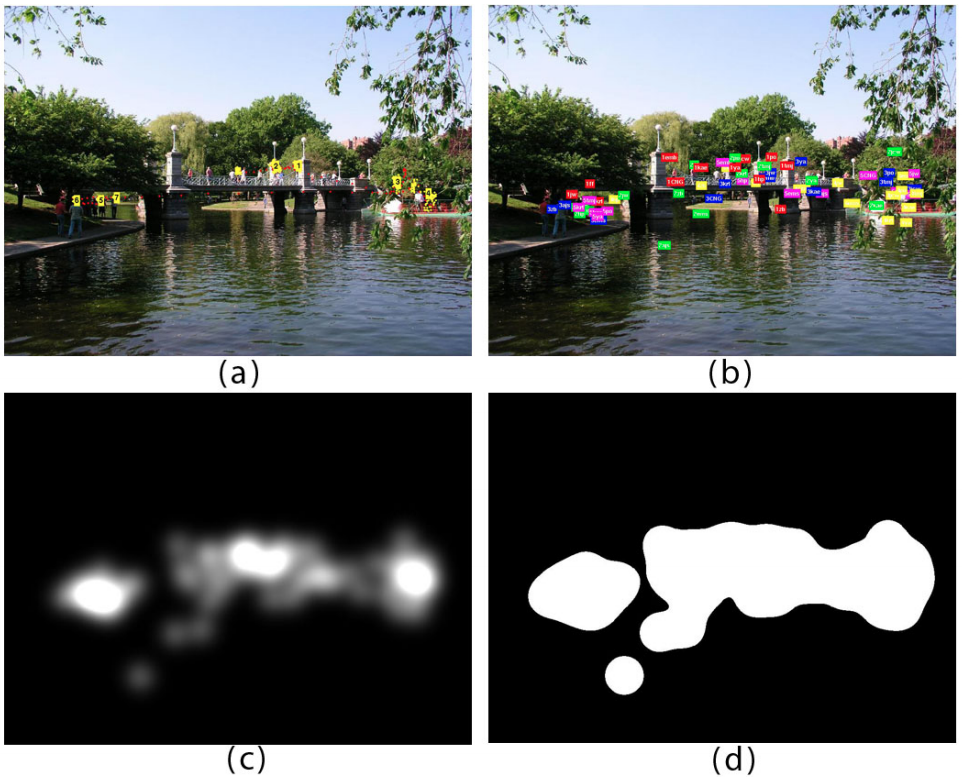
\includegraphics[width=1\textwidth]{\ImgPath/rys/mit300.png}
		\caption{Zbiór danych zebranych przez zespół z MIT. Zawiera on 1003 obrazy obejrzane przez 15 badanych. Miejsca skupienia uwagi zostały zaznaczone dla każdego badanego (b). Mapa istotności została wygenerowana poprzez użycie filtru Gaussa (c). Można również wygenerować mapy pokazujące najbardziej istotne 20 procent obrazu (d).}
		\label{mit}
	\end{figure}

	\section{Wykrywanie istotnych obiektów}
	Innym zdefiniowanym problemem jest wykrywanie istotnych obiektów (salient object detection), który obejmuje wykrywanie najbardziej wyróżniających się obiektów. Wykorzystanie tego algorytmu to m. in. opisywanie obrazów, wykrywanie obiektów, segmentacja obrazów, streszczanie wideo oraz identyfikacja ludzi. Od przewidywania istotności różni się tym, że poszukuje istotnych obiektów, a nie punktów skupienia uwagi. Historia algorymtów wykrywania istotnych obiektów jest dosyć krótka, początkowo przeważały metody oparte o cechy niskopoziomowe oraz heurystyki(np. kontrast kolorów). Obecnie najczęściej stosuje się metody oparte o uczenie głębokie. Wykorzystuje się splotowe sieci neuronowe, takie jak FCN oraz sieci oparte o kapsuły.

	\section{Wykrywanie współistotnych obiektów}
	Zagadnienie wykrywania współistotnych obiektów (co-salient object detection) stara się wykryć występowanie powtarzalnych oraz istotnych (w sensie postrzegania przez człowieka) regionów w grupie powiązanych ze sobą obrazów. Wykrywanie współistotnych obiektów znajduje swoje zastosowanie jako element przygotowania danych w wielu aplikacjach, takich jak wspólna segmentacja kilku obrazów lub filmu, lokalizacja obiektów, analiza nagrań z kamer bezpieczeństwa oraz wyszukiwanie za pomocą obrazów. 

	Algorytmy wykrywania współistotnych obiektów można podzielić za względu na reprezentacje cech. Duża część algorytmów, np. \cite{ChangLL11}, wykorzystuje cechy niskiego poziomu, takie jak histogramy koloru, filtry Gabor oraz deskryptory SIFT. Metody te zakładają, że współwystępujące obiekty są ze sobą spójne na poziomie cech niskiego poziomu. Kolejna grupa metod, np. \cite{midfeatex}, używa dodatkowo cech średniego poziomu w celu wykrywania współistotnych obiektów. Te metody korzystają zazwyczaj z wyników algorytmów wykorzystujących cechy niskiego poziomu i traktują je jako cechy średniego poziomu, zakładając spójność tych cech w grupie obrazów. Obecnie najwięcej algorytmów, np. \cite{highfeatex}, stosuje cechy wysokiego poziomu, zakładając ich spójność w grupie zdjęć. W ramach algorytmów wykrywania współistotnych obiektów za cechy niskiego poziomu uważa się zazwyczaj te cechy, które odnoszą się do wartości pojedynczych pikseli. Cechy średniego poziomu odnoszą się do map generowanych przez istniejące metody wykrywania współistotnych obiektów. Cechy wysokiego poziomu odnoszą się do cech zawierające znaczące informacje o danych. Dotyczy to najczęściej cech otrzymywanych z warstw głębokich sieci splotowych. 
	

	\begin{figure}[h]
		\centering
		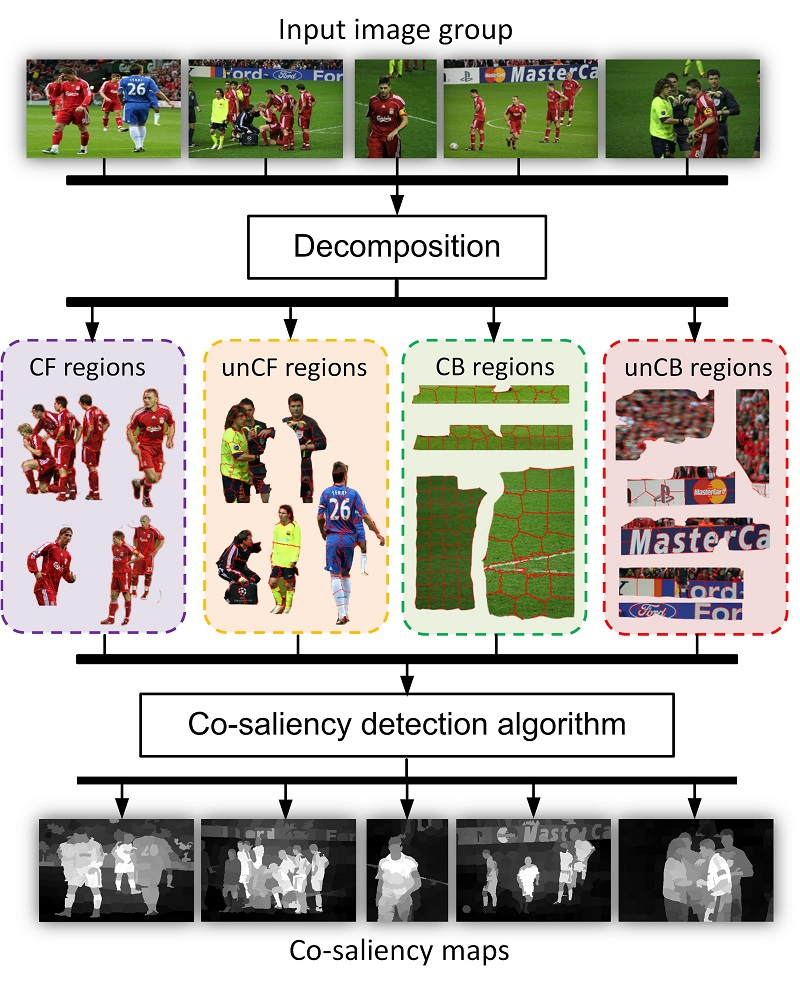
\includegraphics[width=0.6\textwidth]{\ImgPath/rys/cosaliency.png}
		\caption{Przykład podziału grupy obrazów na obszary powtarzające się. Zadaniem algorytmu wykrywania współistotnych obiektów jest stworzenie mapy współistotności pokazującej wspólne obszary istotności. Źródło obrazu: \cite{10.1145/3158674}}
		\label{co}
	\end{figure}

	\section{Przegląd metodyki}
	W zakresie wykrywania współistotnych obiektów wyróżnia się trzy podejścia do tworzenia algorytmów: podejście oddolne, podejście łączące oraz podejście oparte na uczeniu.

	\begin{figure}[h]
		\centering
		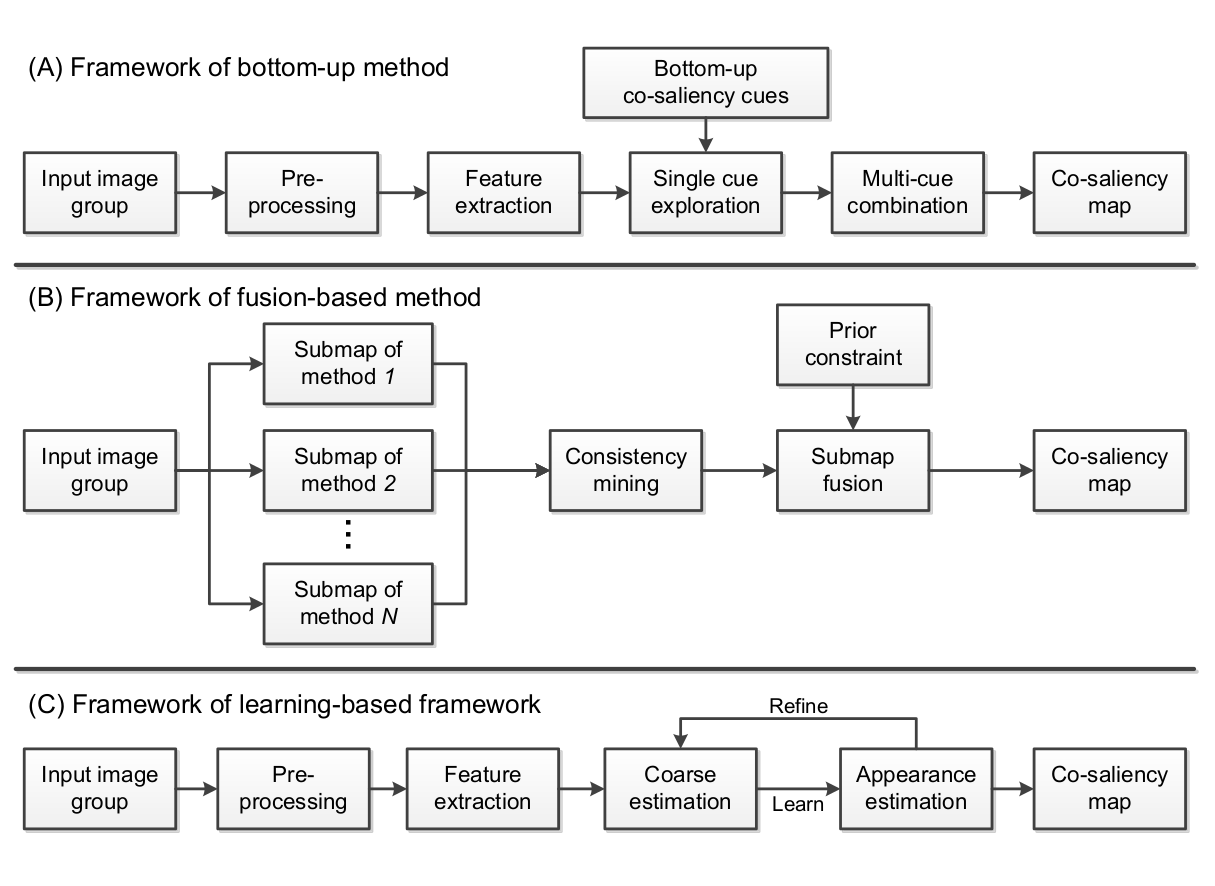
\includegraphics[width=1\textwidth]{\ImgPath/rys/cosal_met.png}
		\caption{Podział algorymtów wykrywania współistotnych obiektów. Źródło obrazu: \cite{10.1145/3158674}}
		\label{pod}
	\end{figure}

	\subsection{Podejście oddolne}
	Pierwsza z omawianych metod skupia się na określeniu wyniku dla każdego pikseli w grupie obrazów korzystając z wcześniej określonych metryk istotności. Na rysunku \ref{pod} (A) przedstawiony jest schemat blokowy algorytmu wykorzystującego podejście oddolne. Składa on się takich kroków, jak: przygotowanie danych, wyodrębnienie cech, analiza pojedynczych metryk istotności oraz analiza kombinacji wielu metryk. Krok przygotowania danych obejmuje podział obrazu wejściowego na pojedyncze obiekty (np. piksele, klastry pikseli lub segmenty superpikseli). Następnie wyodrębniane są cechy każdego obiektu w celu ustalenia jego właściowści w oparciu o wcześniej stworzone metryki istotności. Ostatnim krokiem jest połączenie map istotności dla całej grupy obrazów za pomocą metryk współistotności, których stworzenie jest głównym problemem podzas tworzenia tego rodzaju metod. W ogólności metryki współistotności można opisać jako:

	$$
		\text{Co-saliency} = \text{Saliency} \times \text{Repeatedness}
	$$

	% Co w tłumaczeniu na język polski można zapisać:

	% $$
	% 	Współwystępowanie = Istotność \times Powtarzalność
	% $$

	Do analizy metryk używane są różne techniki, m. in. matrix factorization oraz pattern mining. 

	Jedną z najczęściej stosowanych metod oddolnych, jest taka, która wykorzystuje mechanizm klasteryzacji oparty o trzy metryki istotności. Dla każdego klastra $t$ jego współwystępowanie określone jest jako:

	\begin{equation}
		\text{Co-saliency}^t = Cue^t_{Con} \times Cue^t_{Spa} \times Cue^t_{Corr}
	\end{equation}
	gdzie:

	\begin{equation}
		Cue^t_{Con} = \sum_{\tau \neq t} \frac{n^\tau}{N}\left(\|\mathbf{u}^\tau - \mathbf{u}^t\|_2\right)
	\end{equation}
	\begin{equation}
		Cue^t_{Spa} = \frac{1}{n^t}\sum_{p \in C_t} \mathcal{N}\left(\|\mathbf{z}_p - \mathbf{o}_p\|_2|0,\sigma^2\right)
	\end{equation}
	\begin{equation}
		Cue^t_{Corr} = 1/\left(\text{Var}\left(\mathbf{q}^t\right)+1\right)
	\end{equation}
	gdzie $Cue^t_{Con}$, $Cue^t_{Spa}$ i $Cue^t_{Corr}$ oznaczają odpowiednio metryki kontrastu, przestrzeni oraz zgodności. $\mathbf{u}^t$, $n^t$ oraz $\mathbf{q}^t$ oznaczają odpowiedznio centrum klastra, liczbę pikseli oraz dystrybujcę klastra $C_t$. Estymator jądrowy gęstości o jądrze normalnym $\mathcal{N}(\cdot)$ służy do wyznaczenia metryki euklidesowej pomiędzy $\mathbf{z}_p$ (współrzędnymi piksela p) oraz współrzędnymi centrum odpowiedniego obrazu $\mathbf{o}_p$. $\text{Var}\left(\mathbf{q}^t\right)$ oznacza wariancję histogramu $\mathbf{q}^t$. Algorytm jest dokładniej opisany w \cite{bott}.

	Metody wykorzystujące podejście oddolne są najczęściej używane w zadaniu wykrywania współistotnych obiektów. Problemem tych metod jest jednak potrzeba ręcznego stworzenia odpowiednich metryk istotności. Metryki te są najczęściej zbytnio dostosowane do konkretnego zadania i słabo radzą sobie z generalizacją.

	\subsection{Podejście łączące}
	Metody stosujące to podejście starają się wydobyć informacje o współwystępowaniu z wyników istniejących już algorytmów wykrywania istotnych lub współistotnych obiektów. Łączą te wyniki oraz zdobytą wiedzę, aby generować wynikowe mapy współistotności. Na rysunku \ref{pod} (B) przedstawiony jest schemat blokowy algorytmu wykorzystującego podejście łączące. Pierwszym krokiem jest wygenerowanie map poprzez użycie istniejących algorytmów na danym zbiorze obrazów. Następnie poszukuje się powtarzalności pośród wygenerowanych map. W celu wyznaczenia wag połączenia map stosowane są ograniczenia ułatwiające ten proces. W ostatnim kroku wyznaczone wcześniej mapy łączone są w celu wygenerowania ostatecznych map współistotności:

	$$
	\text{Co-saliency} = \sum_i \text{Weight}_i \cdot \text{Submap}_i
	$$

	Typowym podejściem wykorzystującym to podejście jest \cite{midfeatex}. Mając macierz cech $\mathbf{H} = [\mathbf{H}^1, \mathbf{H}^2, \dots, \mathbf{H}^K]^T \in R^{M \times D}$, $K$, $M$ oraz $D$ oznaczają odpowiednio liczbę obrazów, liczbę wyznaczonych map dla każdego obrazu oraz wymiar danej cechy. Powtarzalność pomiędzy tymi mapami może być wyznaczona jako:

	\begin{equation}
		\arg\min_{\mathbf{L}, \mathbf{E}} \left(\|\mathbf{L}\|_* + \lambda\|\mathbf{E}\|_1\right)
	\end{equation}

	\begin{equation}
	\mathbf{H} = \mathbf{L} + \mathbf{E}
	\end{equation}
	gdzie $\|\cdot\|_*$ oznacza normę macierzy, a $\|\cdot\|_1$ jej normę $l_1$. Macierz $\mathbf{E}$ jest macierzą błędów między macierzą $\mathbf{H}$ oraz macierzą rang $\mathbf{L}$, gdzie $\mathbf{E}^k=[\mathbf{e}^k_1, \mathbf{e}^k_2, \dots, \mathbf{e}^k)M]^T \in R^{M \times D}$ jest macierzą błędu $k$-tego obrazu. Zatem waga $w^k_j$ dla $j$-tej mapy $k$-tego obrazu może zostać wyznaczona jako:

	\begin{equation}
	w^k_j = \frac{\exp(\zeta^k_j)}{\sum^M_{j=1}\exp(\zeta^k_j)}
	\end{equation}


	\begin{equation}
		\exp(\zeta^k_j) = -\|e^k_j\|_2
	\end{equation}
	
	Metody wykorzystujące podejście łączące zazwyczaj osiągają wyniki pozwalające sądzić, że są w stanie rozwinąć się korzystając z istniejących algorytmów wykrywania współistotnych obiektów. Kolejnym plusem tej grupy algorytmów jest fakt, że istnieje możliwość dodania ich jako kolejna warstwa w procesie przetwarzania, w którym zaimplementowane są już algorytmy wykrywania współistotnych obiektów. Ich wadą jest jednak to, że opierają swoje działania o istniejące algorytmy wykorzystujące podejście oddolne, powielając wady tej grupy algorymtów.

	\subsection{Podejście oparte o uczenie}
	Trzecią grupą algorymtów są metody oparte na uczeniu. Dążą one do wyuczenia się wzorów współistotności z danej grupy obrazów. Wspomniane wcześniej dwie grupy metod również mogą wykorzystywać uczenie maszynowe podczas konkretnych kroków, ale nie używają tej techniki do wyznaczania mapy współistotności. Na rysunku \ref{pod} (C) przedstawiony jest schemat blokowy algorytmu opartego o uczenie. Cechą charakterystyczną tej metody jest wykorzystanie algorytmu uczenia nienadzorowanego do wyznaczenia początkowej mapy współistotności. Kolejnym krokiem jest iteracyjne uczenie się algorytmu w celu poprawy wyznaczonej mapy współistotności.

	Przykładem z algrytmu z tej grupy może być algorytm opisany w \cite{10.1109/TPAMI.2016.2567393}. Zakładamy, że mamy grupę zdjęć $K_+$ opisaną jako zbiór pozytywny oraz wyszukaną grupę zdjęć $K_-$ opisaną jako zbiór negatywny. Dla każdego obrazu wyznaczamy superpiksele wraz z reprezentacją cech $\mathbf{x}_i^{(k)}$, które traktowane są jako obiekty do klasyfikacji, gdzie $k \in [1, K]$, $K=K_+ + K_-$ oznacza index w zbiorze dla każdego obrazu, a $i \in [1, n_k]$ oznacza indeks superpiksela obiektu dla każdego $k$-zbioru. Funkcja kosztu jest zdefiniowana jako:

	\begin{equation}
		\min_{\mathbf{w},b,\mathbf{y}^{(1)}, \dots, \mathbf{y}^{(K_+)},\mathbf{v}\in[0,1]^n} E(\mathbf{w},b,\mathbf{y}^{(1)}, \dots, \mathbf{y}^{(K_+)},\mathbf{v}) = 
	\end{equation}

	\begin{equation}
		\frac{1}{2} \|\mathbf{w}\|^2_2 + \sum_{k=1}^K \sum_{i=1}^{n_k}v_i^{(k)} L(y_i^{(k)}, g(\mathbf{x}^{(k)}_i;\mathbf{w},b)) + f(\mathbf{v};\lambda, \gamma)
	\end{equation}

	\begin{equation}
	\|\mathbf{y}^{(k)}+1\|_0 \geq 1, k=1,2,\dots,K_+
	\end{equation}
	gdzie $\mathbf{v} = [v_1^{(1)}, \dots, v_{n_1}^{(1)}, v_{1}^{(2)}, \dots, v_{n_2}^{(2)}, \dots, v_{n_k}^{(K)}] \in R^{n}$ oznacza znaczenie wag dla obiektów, $\mathbf{y} = [y_1^{(k)}, y_{2}^{(k)}, \dots, y_{n_k}^{(k)}] \in R^{n_k}$ oznacza etykiety dla obiektu $k$-tego zbioru, $L(y_i^{(k)}, g(\mathbf{x}^{(k)}_i;\mathbf{w},b))$ oznacza funkcję kosztu $\mathbf{x}_i^{(k)}$ dla klasyfikatora SVM $g(\mathbf{x}^{(k)}_i;\mathbf{w},b)$ z~wektorem wag $\mathbf{w}$ oraz parametrem bias b. Ograniczenie powoduje, że będzie istniał przynajmniej jeden pozytywny obiekt dla każdego pozytywnego zbioru. $f(\mathbf{v};\lambda, \gamma)$ jest funkcją regularyzacji.

	W przypadku algorytmów wykrywania współistotnych obiektów tego rodzaju wiedza obiektach współwystępujących poznawana jest przez algorytm w procesie uczenia, zamiast w rezultacie ręcznie zaprojektowanych metryk. Algorytmy uczenia maszynowego są w stanie znaleźć bardziej skomplikowane zależności w danych od człowieka, ponieważ metryki wymyślane przez człowieka są najczęściej nadmiernie dostosowane do konkretnego zadania i mają słabą zdolność generalizacji. Wadą algorytmów opartych o uczenie jest czas potrzebny w etapie treningu.



	\section{Ocena algorytmów}
	Algorytmy wykrywania współistotnych obiektów sprawdzane były najczęściej na czterech publicznych zbiorach danych: Image Pair \cite{ImagePair}, iCoseg \cite{iCoseg}, MSRC \cite{MSRC} oraz Cosal2015 \cite{cosal2015}. Przykładowe obrazy z każdego zbioru przedstawione są na rysunku \ref{ds}. 

	\subsection{Zbiory danych}

	\begin{figure}[h]
		\centering
		\includegraphics[width=1\textwidth]{\ImgPath/rys/datasets.png}
		\caption{Przykładowe obrazy ze zbiorów danych służących do oceny algorytmów wykrywania współistotnych obiektów. Źródło obrazów: \cite{10.1145/3158674}}
		\label{ds}
	\end{figure}

	Zbiór danych Image Pair \cite{ImagePair} zawiera 105 par obrazów (razem 210 obrazów) o rozdzielczości 128x100 pikseli. Posiada ręcznie określane wartości prawdy i jest pierwszym zbiorem danych dla zadania wykrywania współistotnych obiektów. Każda z par obrazów zawiera podobne obiekty znajdujące się na różnym tle. W tym zbiorze danych tło jest mniej zróżnicowane niż w innych zbiorach. Obecnie zbiór ten nie jest często używany, ponieważ nie jest wystarczająco wymagający dla nowoczesnych algorytmów.
	
	% \begin{figure}[h]
	% 	\centering
	% 	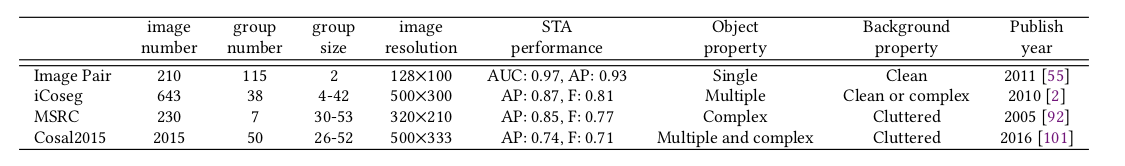
\includegraphics[width=1\textwidth]{\ImgPath/rys/ds_comp.png}
	% 	\caption{Tabela przedstawiająca porównanie zbiorów danych.}
	% 	\label{table}
	% \end{figure}

	% \begin{table}[h]
	% 	\centering
	% 	\resizebox{\textwidth}{!}
	% 	{\begin{tabular}{c||cccccccc}
	% 	\hline
	% 			   	& Liczba obrazów & Obrazy w grupie 	& Wielkość grupy 	& Rozdzielczość obrazów 	& SOTA 			& Obiekty 	& Tło 			& Rok publikacji \\ \hline \hline
	% 	Image Pair 	& 210            & 115     					& 2                 & 128$\times$100        		& AUC: 0.97, AP: 0.93   & Pojedyncze       			& Jednolite 					& 2011 \\
	% 	iCoSeg     	& 643            & 38     					& 4-42              & 500$\times$300        		& AP: 0.87, F: 0.81     & Wiele        				& Różne	& 2010 \\
	% 	MSRC 		& 230            & 7     					& 30-53             & 320$\times$210        		& AP: 0.85, F: 0.77     & Złożone        			& Skomplikowane 					& 2005 \\
	% 	CoSal2015  	& 2015           & 50    					& 26-52             & 500$\times$333      		& AP: 0.74, F: 0.71     & Wiele oraz złożone        & Skomplikowane 					& 2016 \\  \hline
	% 	\end{tabular}}
	% \end{table}

	Zbiór iCoseg \cite{iCoseg} jest otwartym zbiorem danych. Posiada 38 grup obrazów (643 razem), jak również wartości prawdy dobrane ręcznie dla każdego piksela. W odróżnieniu od zbioru Image Pair grupy zawierają od 4 do 42 obrazów. Obrazy w tym zbiorze charakteryzują się najczęściej zróżnicowanym tłem oraz kilkoma obiektami na obrazie. Zbiór ten jest jednym z najczęsciej używanych podczas ewaluacji algorytmów wykrywania współistotnych obiektów.

	Kolejnym często używanym zbiorem jest zbiór MSRC \cite{MSRC}. Zawiera on 8 grup (razem 240 obrazów) wraz z prawdą ręcznie dobraną dla każdego piksela. Grupy obrazów to np. samoloty, rowery lub samochody. Istnieje również grupa zawierająca trawę, jednak nie jest ona zazwyczaj używana w zadaniu wykrywania współistotnych obiektów, ponieważ ich nie zawiera.

	Nowszym zbiorem danych jest Cosal2015 \cite{cosal2015}. Posiada on 50 grup zdjęć (2015 razem) zebranych z konkursu ILSVRC2014 oraz filmów w serwisie YouTube. Tła obrazów w tym zbiorze są mocno zróżnicowane. Dodatkowo często na jednym obrazie znajduje się kilka obiektów istotnych, których część nie występuje na innych obrazach w grupie.
 
	
	Obecnie zaproponowane zsotały dwa nowe zbiory danych. Zbiór CoSOD3k \cite{fan2020rethinking} zawiera 3316 obrazów ze zbioru ILSVRC, podzielonych na 160 grup. Obrazy posiadają opisy przyporządkowujące je do klas oraz 13 superklas. Zbiór ten różni się od wcześniej opisanych tym, że posiada bardziej realistyczne sceny, na których trudniej wykryć obiekty. Posiada on również obrazy, na których znajdują się dwie lub trzy instancje obiektu. W tabeli powyżej zbiory danych porównane są pod kątem wielkości obiektu oraz liczby instancji.

	\begin{table}[]
		\caption{Porównanie liczby instancji obiektów w podanych zbiorach danych.}
		\begin{tabular}{c||ccc||ccc}
		\hline
				   & \multicolumn{3}{c||}{Wielkość instancji/obiektu}             & \multicolumn{3}{c}{Liczba instancji} \\
				   & duża (\textgreater{}30\%) & średnia & mała (\textless{}5\%) & 1          & 2        & 3       \\ \hline
		MSRC       & 123                       & 109     & 1                     & 233        & -        & -        \\
		iCoSeg     & 171                       & 385     & 87                    & 643        & -        & -        \\
		Image Pair & 60                        & 147     & 3                     & 105        & -        & -        \\
		CoSal2015  & 616                       & 1161    & 238                   & 2015      & -        & -        \\ \hline \hline
		CoSOD3k    & 439                       & 3173    & 1303                  & 2371       & 644      & 334      \\ \hline
		\end{tabular}
	\end{table}

	W ramach artykułu \cite{zhang2020gradientinduced} zespół proponuje kolejny zbiór danych nazwany CoCA. Stworzenie nowego zbioru wynika z braku odpowiednio wymagających istniejących danych. Wcześniejsze zbiory danych zawierają jedynie jeden istotny obiekt na każdym z obrazów, co czyni z ich wykrycia zadanie łatwe dla algorytmów wykrywania istotnych obiektów, znosząc potrzebę użycia algorytmu do wykrywania współistotnych obiektów. Ważna jest zatem odpowiednia złożoność zbiorów danych, tzn. kilka obiektów istotnych na jednym obrazie, ponieważ z takie dane będą przetwarzane przez algorytmy wykrywania wpółistotnych obiektów w aplikacjach komercyjnych. Na rysunku \ref{CoCA} przedstawione są przykładowe obrazy ze zbioru danych CoCA, pokazujące obrazy zawierające kilka obiektów istotnych. 

	\begin{figure}[h]
		\centering
		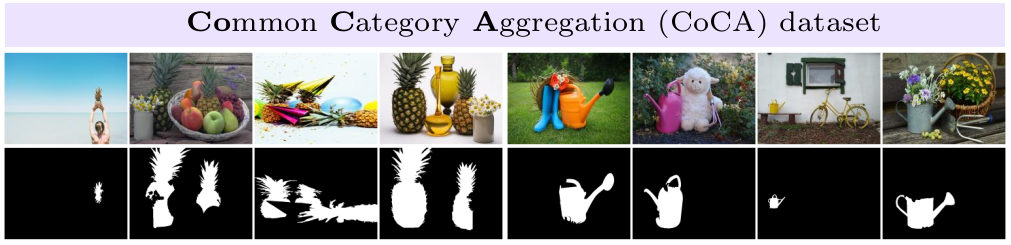
\includegraphics[width=1\textwidth]{\ImgPath/rys/CoCA.png}
		\caption{Przykłady obrazów ze zbioru danych CoCA. Źródło obrazu: \cite{zhang2020gradientinduced}}
		\label{CoCA}
	\end{figure}


	\subsection{Miary oceny}
	Oceny algorytmów wykrywania współistotnych obiektów można dokonać za pomocą sześciu przyjętych miar: krzywej PR (precyzja-czułość), średniej precyzji (AP), krzywej miary F, średniej miary F (mF), krzywej ROC oraz miary AUC. 

	Krzywa PR oraz miara AP wyznaczane są poprzez podział pikseli w mapie istostności na istotne oraz nieistotne. W rezultacie miara czułości zestawiona z miarą precyzji tworzy krzywą PR. Pole pod krzywą wyznacza miarę średniej prezyzji (AP). Krzywa ROC jest wyznaczana w podobny sposób, brane pod uwage są jednak miary liczby fałszywie dodatnich oraz prawdziwie dodatnich przykładów. Miara AUC wyznaczana jest jako pole pod krzywą ROC. Precyzja i czułość zdefiniowane są jako:

	\begin{equation}
		Precision = \frac{TP}{TP + FP}, \; Recall = \frac{TP}{TP + FN}
	\end{equation}

	gdzie TP, FP oraz FN oznaczają odpowiednio liczbę przypadków prawdziwie dodatnich, fałszywie dodatnich oraz fałszywie ujemnych. Odpowiadająca miara F-score zdefiniowana jest jako:

	\begin{equation}
		F_{\beta} = \frac{(1 + \beta^2)\cdot Precision \cdot Recall}{(\beta^2 \cdot Precision) + Recall}
	\end{equation}

	gdzie sugerowana wartość $\beta^2 = 0.3$. Wartości progowe oraz wartości miary F-score tworzą krzywą F-measure. 

	Spośród wcześniej wymienionych miar krzywe ROC, PR oraz F-measure przekazują więcej informacji niż odpowiadające im miary. Pozwalają na sprawdzenie jak zmienia się wartość miary w zależności od czynników znajdujących się na osiach. W ramach porówniania jakości różnych algorytmów stosuje się najczęściej miary AP, średnią F-score oraz AUC, ponieważ pozwalają w zwięzły sposób ocenić jakość algorytmu. 


\chapter{Wybrane metody wykrywania współistotnych obiektów}
\textcolor{red}{\textbf{TODO - 31.10.2020}}
\section{Gradient-Induced Co-Saliency Detection}

Jedną z dwóch metod wykrywania współistotnych obiektów jest metoda Gradient-Induced Co-Saliency Detection (GICD) \cite{zhang2020gradientinduced}, która wykorzystuje schematy zachowań wykształcone przez człowieka.

\subsection{Inspiracja ludzkim zachowaniem}
Zespół zajmujący się omawianą w tej sekcji metodą pracę nad algorytmem rozpoczął od zadania sobie pytania: jak ludzie rozpoznają współistotne obiekty w grupie obrazów? Najczęściej pierwszym etapem jest przejrzenie grupy obrazów, następnie podsumowanie wspólnych właściowści współistotnych obiektów za pomocą wiedzy ogólnej oraz rozpoznanie współistotnego obiektu dla każdego z obrazów. Proces ten został przedstawiony na pierwszej części rysunku \ref{GICDhuman}. Opierając się na schemacie ludzkiego zachowania, zespół opracował sieć podzieloną na dwa etapy. Właściowści współdzielone przez istotne obiekty z danej grupy uzyskiwane są poprzez wyuczoną wcześniej sieć spolotową. Następnie dla każdego obrazu wykorzystywany jest Gradient Inducing Module (GIM), w celu imitacji zachowania człowieka podczas porównywania konkretnej sceny do wiedzy ogólnej dotyczącej obiektów współistotnych.

\begin{figure}[h]
	\centering
	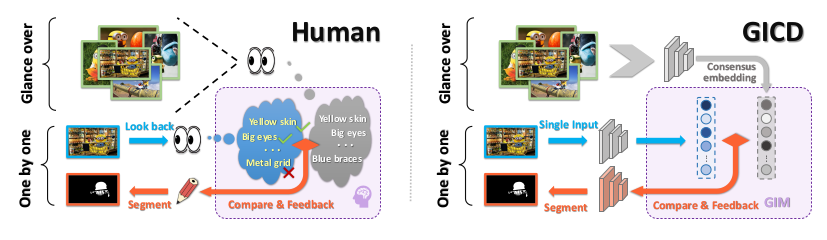
\includegraphics[width=1\textwidth]{\ImgPath/rys/gicdhuman.png}
	\caption{Metoda GICD została oparta na mechanizmach pochodzących od człowieka. Źródło obrazu: \cite{zhang2020gradientinduced}}
	\label{GICDhuman}
\end{figure}

W GIM jako pierwsze wyznaczane jest podobieństwo między cechami pojedynczego obrazu oraz cechami ogólnymi. W trakcie uczenia, poprzez propagację wsteczną, wyznaczane są gradienty podobieństwa. Wykorzystywana do tego jest najwyższa warstwa splotowa. Wysokie wartości gradientów oznaczają, że odpowiadające im postaci jądra mają pozytywny wpływ na wyniki podobieństwa, zatem poprzez zwiększenie wag tych postaci jądra algorytm wybierze cechy związane z współistotnością. Dodatkowo, w celu lepszego opisania współistotnych obiektów w każdym z poziomów dekodera, zaproponowany został Attention Retaining Module (ARM). Moduł ten łączy poszczególne pary dekoder-enkoder. Jako podstawa sieci użyta jest sieć Feature Pyramid Network (FPN) \cite{lin2017feature}.

Problemem występującym podczas trenowania algorymów wykrywania współistotnych obiektów jest brak odpowiednich zbiorów danych. Z tego powodu trenowanie przeprowadzane jest na zbiorach przeznaczonych do segmentacji obrazów, takich jak Microsoft COCO. Wadą tego rozwiązania jest to, że w takich zbiorach nie wszystkie oznaczone obiekty są istotne. Z tego powodu została zapronowana nowa strategia trenowania, pozwalająca na poszerzenie istniejących zbiorów danych bez dodawania nowych opisów. 

\begin{figure}[h]
	\centering
	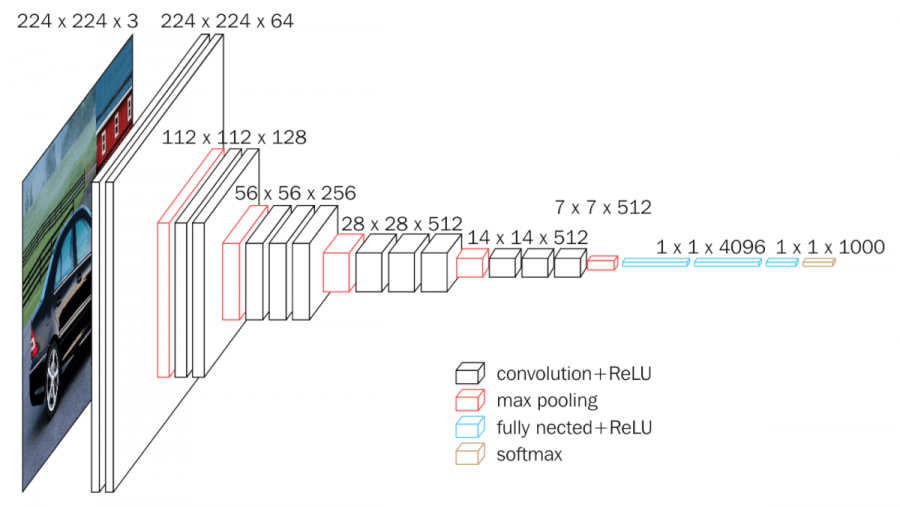
\includegraphics[width=1\textwidth]{\ImgPath/rys/vgg16.png}
	\caption{Architektura sieci VGG. Zawiera ona 16 warstw CONV/FC. Stosowane są w niej jedynie filtry 3x3 oraz próbkowanie 2x2. Sieć posiada 138 milionów parametrów oraz zajmuje 93 MB pamięci (jedynie dla propagacji w przód) dla jednego obrazu o wymiarach [224x224x3].}
	\label{vgg}
\end{figure}


\subsection{Wyuczenie współdzielonych cech}
Mając grupę obrazów $\mathcal{I}=\{I_n\}_{n=1}^N$, aby zlokalizować współistotne obiekty na każdym z obrazów, konieczne jest wyznaczenie cech współdzielonych przez wszystkie obiekty współistotne opartych na wiedzy ogólnej. W celu wyznaczenie tych cech wykorzystywana jest wyuczona wcześniej sieć splotowa. Głębokie sieci splotowe mogą być użyte jako narzędzie ekstrakcji cech, wyuczonych wcześniej do zadania rozpoznawania obrazów. W przypadku tego rozwiązania użyta została wcześniej wyuczona sieć głęboka VGG-16 \cite{SimonyanZ14a} (rysunek \ref{vgg}), z której usunięta została ostatnia warstwa Softmax. Sieć ta w dalszej części pracy oznaczana jest jako $\mathcal{F}(\cdot)$. Na początku wyznaczana jest reprezentacja $e_n=\mathcal{F}(I_n)\in\mathds{R}^d$ każdego obrazu $I_n$, gdzie $d$ oznacza wymiary ostatniej w~pełni połączonej warstwy sieci. Reprezentacja wspólnych cech $e^\dagger$ wyznaczana jest jako $e^\dagger = Softmax\left(\sum^{N}_{n=1}e_n\right)$.

\begin{figure}[h]
	\centering
	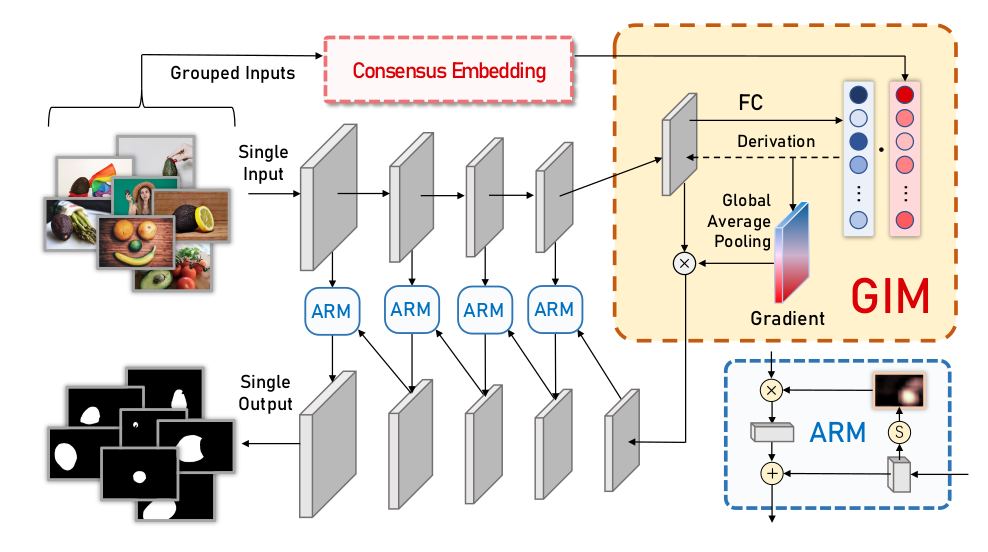
\includegraphics[width=1\textwidth]{\ImgPath/rys/gicosadNet.png}
	\caption{Potok przetwarzania obrazów metodą Gradient-Induced Co-saliency Detection (GICD). Źródło obrazu: \cite{zhang2020gradientinduced}}
	\label{GICDnet}
\end{figure}

\subsection{Gradient Inducing Module}
Po wyznaczeniu reprezentacji wspólnych cech $e^\dagger$ grupy obrazów $\mathcal{I}$ dla każdego obrazu, konieczne jest skupienie się na wyznaczeniu opisujących cech pokrywających się z opisem wspólnych cech. Wysokopoziomowe warstwy sieci splotowych posiadają informacje dotyczące właściwości przestrzennych obiektów, co opisane zostało w \cite{Selvaraju_2019}. Grupy cech sieci splotowej $\mathcal{F}(\cdot)$ oznaczone zostały jako $\{F^1, F^2, ..., F^5\}$. Poziom opisowości cech w sieci neuronowej może zostać zmierzony poprzez wyliczenie gradientu wyznaczone podczas optymalizacji celu. W związku z tym, zaproponowany został Gradient Inducing Module (GIM) zwiększający opisowość cechy poprzez przetworzenie informacji dotyczących gradientu. Enkoder sieci FPN posiada takie same parametry jak sieć wyznaczająca reprezentację wspólnych cech, może on zatem przedstawić obraz w przestrzeni takiej samej jak wspólna reprezentacja cech $e^\dagger$. Dla reprezentacji n-tego obrazu $e_n$, podobieństwo $c_n$ pomiędzy $e_n$, a odpowiadającej jej $e^\dagger$ może zostać zdefiniowane jako iloczyn $c_n = e_n^Te^\dagger$. Następnie wyznaczony zostaje gradient $G_n$ uwzględniając ostatnią warstwę splotową $F^5\in\mathds{R}^{w\times h\times c}$:

\begin{equation}
 G_n = ReLU \left(\frac{\partial c_n}{\partial F^5_n}\right) \in \mathds{R}^{w\times h\times c}.
\end{equation}

W tej częściowej propagacji wstecznej, gradient $G_n$ pokazuje wagę odpowiadającej mu pozycji w końcowej wartości podobieństwa. Im bardziej zostanie zwiększona wartość aktywacji oraz gradient, tym bardziej zbliżona będzie pojedyncza reprezentacja cech $e_n$ do wspólnej $e^\dagger$. W związku z tym, waga postaci jądra dla poszczególnego obiektu może zostać zmierzona poprzez średnią gradientów cech. Wagi dla poszczególnych kanałów mogą zostać wyznaczone poprzez globalne uśrednienie (GAP), oznaczone $w_n = GAP(G_n) = \frac{1}{wh}\sum_i\sum_jG_n$, gdzie $i = 1, \dots, w$ oraz $j = 1, \dots, h$.  Po wyznaczeniu wagi można dostosować wysokopoziomową cechę $F_n^5$ przez dopasowanie wagi do każdej z postaci jądra $\tilde F_n^5 = F_n^5 \otimes w_n$, gdzie $\otimes$ oznacza iloczyn Hadamarda. Bez użycia modułu GIM jądra będą koncentrowały się się na wszystkich istotnych obiektach. Moduł GIM pozwala poprzez użycie informacji o gradientach na zawężenie działania jąder do jedynie współistotnego obiektu.

\subsection{Attention Retaining Module}

Użycie GIM pozwala na dostosowanie wysokopoziomowych cech z użyciem gradientu. Podczas dekodowania, własności tych wysokopoziomowych cech będą stopniowo tracone podczas transmisji poprzez warstwy. W związku z tym zaproponowany zostaje Attention Retaining Module (ARM), łączący poszczególne pary enkoder-dekoder. Pozwala on sieci skupić się na obiektach współistotnych, pomijając pozostałe nieważne obiekty. Jako pierwsza mapa o niskiej rozdzielczości $S_n^5$ brana jest średnia dla kanału dla $\tilde F_n^5$. $P_n^5$ oznacza zredukowaną do 64 kanałów $\tilde F_n^5$. Proces dekodowania ARM można zapisać:

\begin{equation}
\begin{cases}
	\tilde F_n^i = (S_n^{i+1}) \uparrow \astrosun F_n^i \\
	P_n^i = \epsilon^i \left(\left(P_n^{i+1}\right)\uparrow+\mathcal{R}^i\left(\tilde F_n^i\right)\right), i \in {4, 3, 2, 1}, \\
	S_n^i = \mathcal{D}^i (P^i_n)
\end{cases}
\end{equation}
gdzie $(\cdot)\uparrow$ jest operacją zwiększenia próbkowania. $\mathcal{R}^i\left(\cdot\right)$ składa się z dwóch warstw splotowych oraz redukuje rozszerzone cechy $\tilde F_n^i$ do 64 kanałów. $\epsilon^i(\cdot)$ oznacza dwie odpowiadające warstwy konwolucyjne z 64 jądrami, pochodzące z dekodera. $\mathcal{D}^i(\cdot)$ pozwala na predykcje poprzez dwie warstwy splotowe wraz z warstwą sigmoidalną. Ostatnia z $S^1_n$ odpowiada warstwie wyjściowej.

\subsection{Strategia trenowania Jigsaw}
Jednym z problemów zadania wykrywania współistotnych obiektów, jest to, że nie ma dostatecznie dużej liczby zbiorów pozwalających na trening sieci wykrywających współistotne obiekty. Zdefiniowane są dwa powody tej sytuacji: 1) obrazy te nie posiadają adnotacji klasy, zatem nie pozwalają na uczenie modeli dla grupy obrazów; 2) większość obrazów posiada tylko jeden istotny obiekt. Z tego powodu sieci nie są w stanie działać w przypadku, gdy na obrazie znajduję się kilka istotnych obiektów. Obecnie metody wykrywania współistotnych obiektów uczone są na zbiorach przeznaczonych do segmentacji. To stwarza dwa problemy: 1) opisy obiektów nie są dokładne, przez co sieć nie jest w stanie odpowiednio dokładnie rozpoznać szczegółów; 2) obiekty w takim zbiorze danych nie zawsze są istotne. W~celu uniknięcia tych problemów zaprezentowana zostaje strategia trenowania Jigsaw. Pozwala ona na użycie zbiorów przeznaczonych do wykrywania istotnych obiektów do trenowania sieci przeznaczonych do wykrywania obiektów współistotnych. Na początek klasyfikator dzieli zbiór danych na kategorie i~przypisuje im etykiety klas. Następnie tworzone są mini zbiory składające się z obrazów z kilku kategorii. Podzas tworzenia obrazy przyporządkowywane są do zbiorów tak, żeby w danej grupie były obrazy z obiektami, które nie są współistotne oraz takie, które nie posiadają w ogóle istotnego obiektu. Przykład takiego zbioru jest na rysunku \ref{jigsaw}.

\begin{figure}[h]
	\centering
	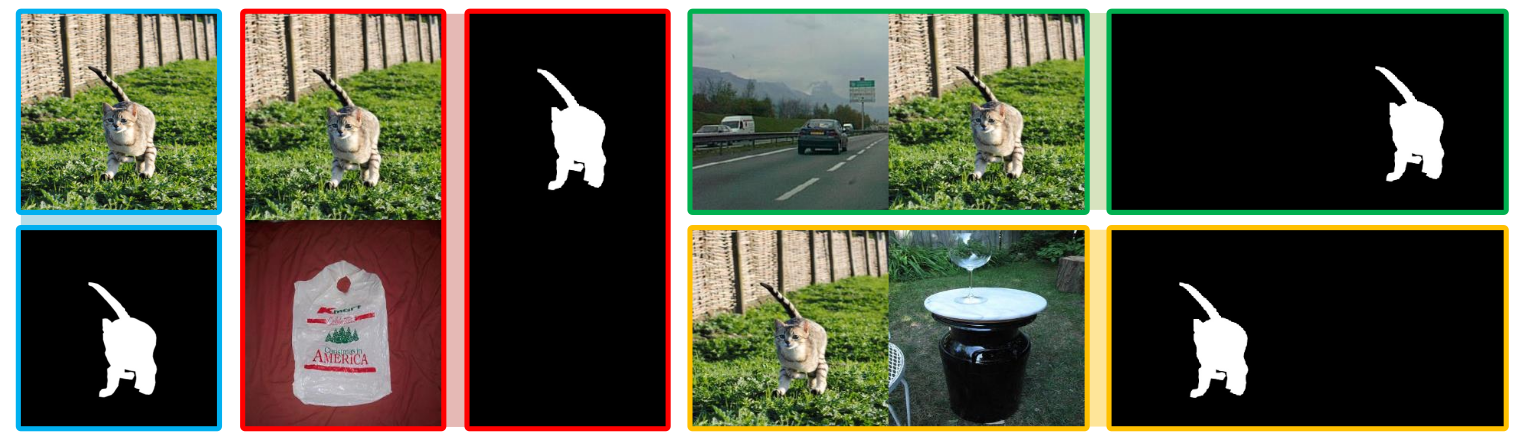
\includegraphics[width=1\textwidth]{\ImgPath/rys/jigsaw.png}
	\caption{Przykład mini zbioru treningowego. Źródło obrazu: \cite{zhang2020gradientinduced}}
	\label{jigsaw}
\end{figure}

Funkcja kosztu zdefiniowana jest jako:

\begin{equation}
	\mathcal{L}(S, G) = 1 - \frac{\sum_cS(c)G(c)}{\sum_c \left[S(c) + G(c) - S(c)G(c)\right]}
\end{equation}

gdzie $S$ jest predykcją, $G$ oznacza wartości prawdziwe. $c$ oznacza pozycje pikseli na obrazie. Pełna funkcja kosztu zdefiniowana jest jako:

\begin{equation}
	L_{total}=\sum^N_{n=1}\sum^4_{i=1}\mathcal{L}(S_n^i, G_n).
\end{equation}

\section{CoEG-Net}
Drugą z metod wykrywania współistotnych obiektów, która osiąga najlepsze wyniki jest metoda CoEG-Net \cite{fan2020rethinking}. Rozszerza ona metodę wykrywania obiektów istotnych EGNet \cite{zhao2019egnetedge} poprzez dodanie informacji dotyczących współskupienia, korzystając z metod uczenia nienadzorowanego.

\subsection{Opis metody}
Dla grupy $N$ zdjęć $\{I^n\}^N_{n=1}$ zadanie wykrywania obiektów współistotnych stara się oddzielić powtarzalne oraz istotne obiekty oraz wygenerować zoptymalizowane mapy współistotności, które przedstwaiają powtarzalne istotne obiekty wsród grupy obrazów. W celu wykrycia współistotnych obiektów zaprezentowano metodę składającą się z dwóch kanałów, które odpowiednio: poszukują wspólnych cech między obrazami oraz znajdują istotne obiekty. Rysunek \ref{coegnet} przedstawia schemat metody, która równolegle wyznacza mapy współskupienia $\{A^n\}^N_{n=1}$ oraz mapy istotności $\{S^n\}^N_{n=1}$. Ostateczne predykcje współistotności uzyskiwane są poprzez wyznaczenie iloczynów Hadamarda $A^n \otimes S^n$ obu kanałów.

W celu wyznaczenia mapy istotności $S^n$ dla obrazu wejściowego $I^n$ użyta jest metoda wykrywania istotności EGNet. Sieć ta nauczona jest na zbiorze treningowym DUTS \cite{duts}. Zadaniem, które jest najważniejsze w kontekście wykrywania współistotności jest wygenerowanie map współskupienie. Zadanie to zostało opisane w następnej sekcji.

\begin{figure}[h]
	\centering
	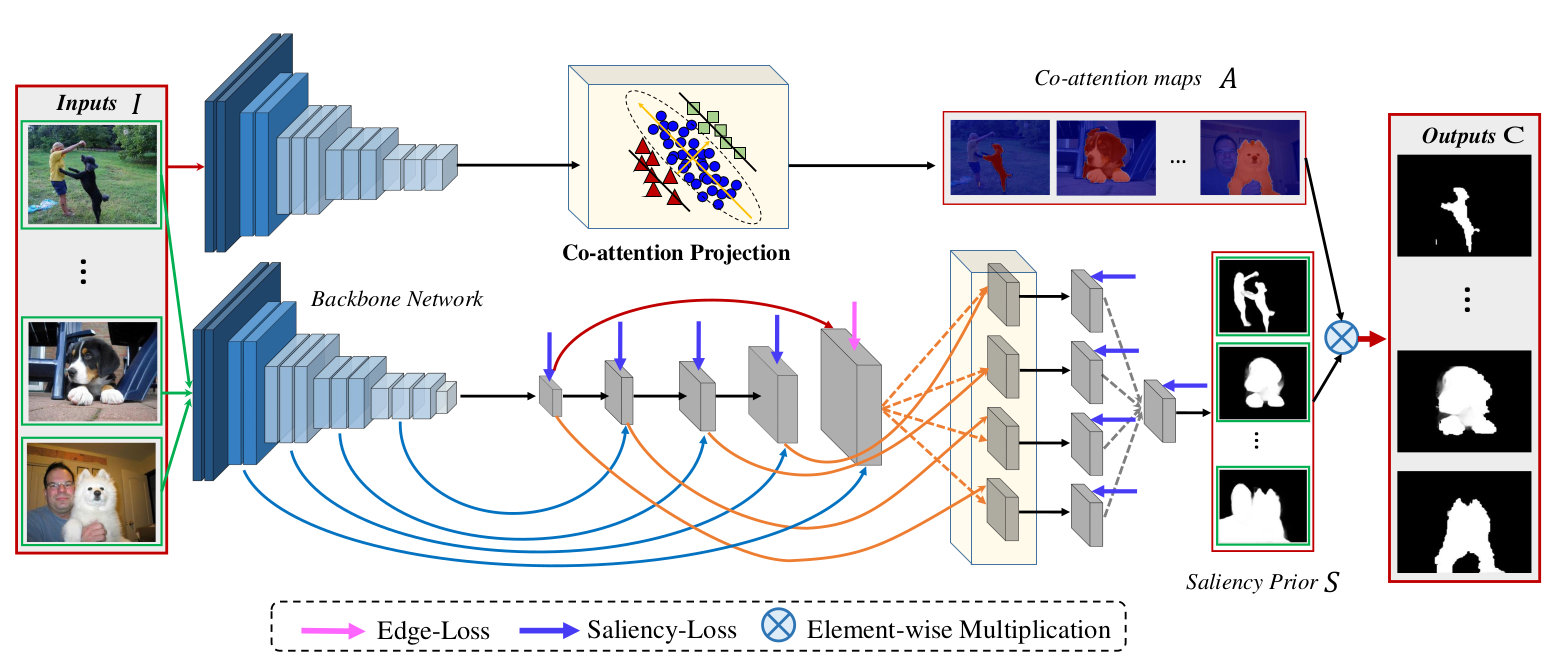
\includegraphics[width=1\textwidth]{\ImgPath/rys/coegnet.png}
	\caption{Metoda CoEG-Net. Składa się ona z dwóch kanałów. Górny wyznacza mapy współskupienia, a dolny wyznacza istotne obiekty na obrazie. Kolejnym krokiem jest wyznaczenie iloczynów Hadamarda obu kanałów. Wynikiem metody są mapy zawierające zaznaczone obiekty współistotne. Źródło obrazu: \cite{fan2020rethinking}}
	\label{coegnet}
\end{figure}

\subsection{Wyznaczanie map współskupienia}
Projekt uczenia opartego na współskupieniu oparty jest na metodzie class
activation mapping (CAM) zaprezentowanej w \cite{cam}. Mając obraz wejściowy $I^n$, odpowiadająca mu mapa aktywacji $X^n$ z ostatniej warstwy sieci splotowej może zostać w łatwości wyznaczona za pomocą klasycznej sieci do rozpoznawania obrazów, np. VGGNet. 

Używając obrazów z etykietą dotyczącą jedynie klasy, metoda CAM tworzy mapy skupienia $M^n_c$ dla każdej klasy $c$, używając map aktywacji cech $\{X^n_k\}$.

\begin{equation}
M^n_c = \sum^K_{k=1} w^c_kX^n_k
\end{equation}

gdzie wagi $w^c$ mogą zostać wyznaczone poprzez uczenie nadzorowane z wykorzystaniem etykiet klas. Elementy przestrzenne mapy aktywacji dla klasy $M^n_c$ mogą być niezależnie wyznaczone poprzez użycie wagi $w^c$ oraz specyficznego dla każdego z kanałów deskryptora $X^n$ na pozycji $(i,j)$ jako
\begin{equation}
M^n_c(i,j) = (w^c)^T \cdot x^n(i,j).
\end{equation}


Metoda CAM jest zatem liniową transformacją przekształcającą cechę obrazu $x^n(i,j)$ na specyficzną dla klasy wartość aktywacji $M^n_c(i,j)$, używając do tego wagi $w^c$.

\begin{table}[h]
	\caption{Opis symboli użytych przy opisie metody.}
	\begin{center}
		
		
		\resizebox{\textwidth}{!}{\begin{tabular}{l|l|l|l}
	\hline \hline
	Symbol  & Wymiary & Współrzędne & Znaczenie \\ \hline
	$A^n$   &       $H\times W$     &    $(i, j)$     &   mapa współskupienie obrazu $I^n$      \\ \hline
	$S^n$   &      $H\times W$      &     $(i, j)$    &    mapa istotności obrazu  $I^n$     \\ \hline
	$X^n$   &      $H\times W\times K$  &     $(i, j, k)$    &    akytwacje ostatniej warstwy splotowej     \\ \hline
	$X^n_k$ &      $H\times W$      &    $(i, j)$     &    mapa cech dla kanału w $X^n$     \\ \hline
	$H$     &      $1\times 1$      &    scalar     &    wysokość     \\ \hline
	$W$     &      $1\times 1$      &    scalar     &    szerokość     \\ \hline
	$K$     &       $1\times 1$     &    scalar     &    liczba kanałów cech (głębokość)   \\ \hline
	$x^n(i,j)$	&  	$K\times 1$	&       $k$            &     deskryptor z $X^n$ o współrzędnych $(i,j)$    \\ \hline
	$M^n_c$	&         $H\times W$   &    $(i, j)$     &    mapa skupienia dla klasy $c$     \\ \hline
	$w^c$	&        $K\times 1$    &     $k$    &   wagi danego kanału dla klasy $c$      \\ \hline
	$\bar{x}$ 	&	$K\times 1$	   &       $k$           &    wartość średnia wszystkich $x^n(i,j)$     \\ \hline
	$\hat{x}^n(i,j)$ &	$K\times 1$	   &     $k$             &   znormalizowane $\hat{x}^n(i,j) = x^n(i,j) - \bar{x}$     \\ \hline
	$Cov(\hat{x})$	&	$K\times K$&        -             &    macierz kowariancji dla $\{\hat{x}^n(i,j)\}$     \\ \hline  
	$\xi^*$		&        $K\times 1$    &    $k$     &     pierwsza wartość własna $
	Cov(\hat{x})$    \\ \hline \hline  
	\end{tabular}}
\end{center}

	\end{table}

Niestety podczas wykrywania obiektów współistotnych nie są dostępne etykiety klas. Wagi $w$ muszą być zatem wyznaczone z wykorzystaniem uczenia nienadzorowanego, poprzez wyznaczenie wewnętrznej struktury cech obrazu. Dla obiektów powtarzających się w danej grupie obrazów $\{I^n\}^N_{n=1}$, transformacja powinna być liniowa i zapewniać wysoki poziom aktywacji dla klasy w obszarze znajdowania się obiektu oraz niski poziom aktywacji w innych regionach obrazu. Opisując to inaczej, powinna generować największą wariancję w wyjściowej mapi aktywacji. Uznano, że metoda analizy głównych składowych (PCA) pozwala w najlepszy sposób na wyznaczenie wewnętrznej struktury danych oraz wyjaśnienie wariancji.

Mając zatem grupę obrazów $\{I^n\}^N_{n=1}$ z odpowiadającymi im aktywacjami cech $X^n$ dla każdego obrazu $I^n$, metoda stara się znaleźć transformację liniową dla $X^n$, wyznaczającą mapy aktywacji $\{A^n\}$ posiadające jak największą wariancję. Może to zostać zrealizowane poprzez analizę macierzy kowarancji deskryptorów cech $\{x^n(i,j)\}$. Niech $\bar{x} = \frac{1}{Z}\sum_n\sum_{i,j}x^n(i,j)$, gdzie $Z=N\times H\times W$. Niech średnia dla znormalizowanego deskryptora wynosi $\hat{x}^n(i,j) = x^n(i,j) - \bar{x}$. Macierz kowariancji może zatem zostać zapisana jako:

\begin{equation}
Cov(\hat{x})=\frac{1}{Z}\sum_n\sum_{i,j}(\hat{x}^n(i,j) - \bar{x})(\hat{x}^n(i,j) - \bar{x})^T
\end{equation}


Wtedy szukana transformacja liniowa może zostać wyznaczona poprzez użycie wektora własnego $\xi^*$ odpowiadającego największej wartości własnej macierzy $Cov(\hat{x})$. Można zapisać ją jako:

\begin{equation}
A^n(i,j) = \xi^{*^T} \cdot \hat{x}^n(i,j).
\end{equation}


Rysunek \ref{actmaps} przedstawia mapy aktywacji dla przykładowych klas. 

\begin{figure}[h]
	\centering
	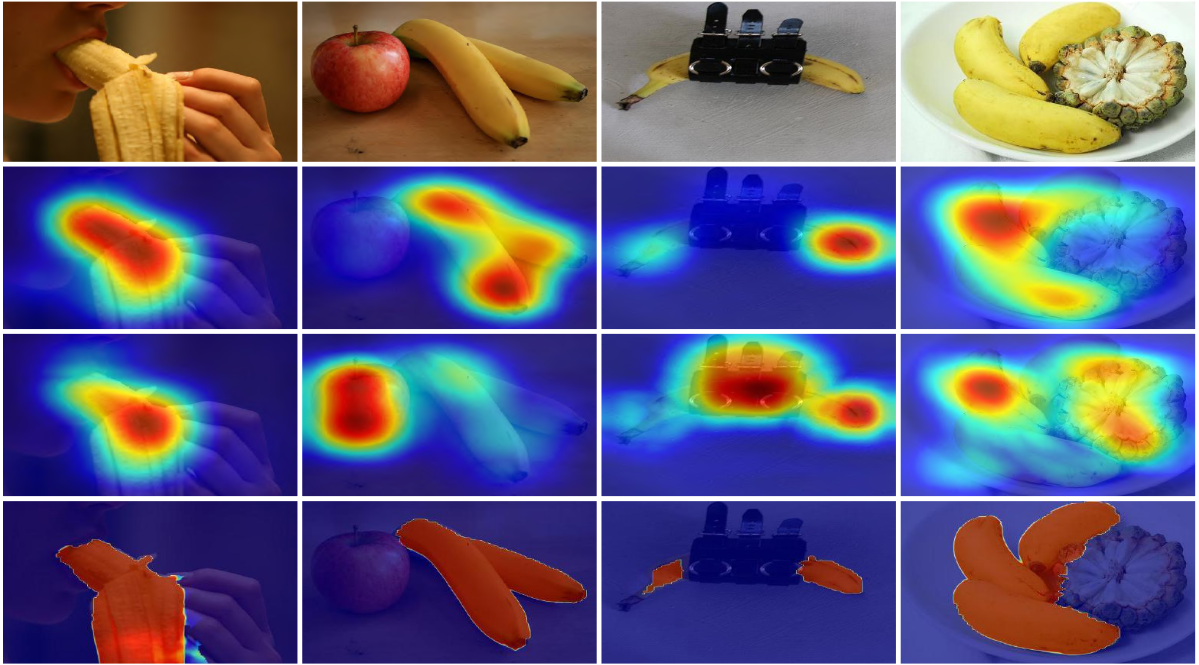
\includegraphics[width=1\textwidth]{\ImgPath/rys/actmaps.png}
	\caption{Wizualizacja wspólnych map aktywacji (drugi i trzeci wiersz), wygenerowanych z użyciem największej i drugiej największej wartości własnej. Czwarty wiersz przedstawia mapy współskupienia $A^n$ dla wybranej klasy - banany. Obrazy pochodzą ze zbioru Cosal2015.}
	\label{actmaps}
\end{figure}


\chapter{Implementacja oraz porównanie wybranych metod}
\textcolor{red}{\textbf{TODO - 30.11.2020, 14.12.2020}}


\chapter{Propozycja własnego algorytmu}
\textcolor{red}{\textbf{TODO - 11.01.2020}}

%   %-----------------
%   % Historia
%   %-----------------

% \section{Historia}
% Pomimo, że pierwsze wzmianki o steganografii, a dokładnie o ukrytych kanałach w 
% odniesieniu do systemów informatycznych notuje się na lata siedemdziesiąte XX 
% wieku \cite{FirstCC}, to przykłady użycia steganografii sięgają starożytności. W 
% literaturze powtarzają się opisy przekazywania tajnej informacji poprzez 
% wytatuowanie jej na ogolonej głowie posłańca, który po odrośnięciu włosów był 
% wysyłany z mało znaczącą wiadomością do armii swojego dowódcy. Każdy kto natknął 
% się na posłańca miał wgląd do nieważnej wiadomości, niepodejrzewając nawet 
% istnienia sekretnej informacji w postaci tatuażu.

% Przykłady z historii odnoszą się także do bardziej współczesnych czasów. Wiele z 
% metod steganografii było stosowanych podczas II Wojny Światowej (np. 
% mikro-kropki) a także w latach Zimnej Wojny. Wiadomo także, że wielu agentów 
% służb wywiadowczych, a szczególnie podwójnych agentów, przekazywało obcym 
% państwom informację wykorzystując steganografię. Przykładem może tu być sprawa 
% szpiega FBI Roberta Hanssena \cite{Hanssen}, który przy pomocy technik 
% steganograficzny przez około dekadę przekazywał tajne informacje służbom KGB.

% Rozdziały \ref{sectionSteganografiaWObiektachMultimedialnych} oraz 
% \ref{chapterSteganografiaWRuchuTCPIP} opisują nowoczesne podejście do 
% steganografii wykorzystujące współczesne kanały informacyjne. 
%   %-----------------
%   % Pojęcia
%   %-----------------
% \section{Pojęcia}
% W celu zdefiniowania kanału steganograficznego oraz opisania transmisji z 
% wykorzystaniem takiego kanału należy omówić jego części składowe:
% \begin{itemize}
% 	\item dane do ukrycia, tajne dane - informacja jaką należy przesłać 
% między uczestnikami komunikacji, tak aby strony trzecie nie miały do niej 
% wglądu,
% 	\item dane nośne, wiadomość zakrywająca - wiadomość, w której ukryte 
% zostaną tajne dane; przesyłanie wiadomości zakrywających musi być dozwolone w 
% danym kanale informacyjnym i nie powinno wzbudzać podejrzeń,
% 	\item funkcja steganograficzna - funkcja przekształcająca dane do 
% ukrycia oraz wiadomość zakrywającą w jedną połączoną wiadomość,
% 	\item dane z ukrytą wiadomością - dane zawierające ukrytą informację a 
% jednocześnie wykazujące cechy danych nośnych,
% 	\item nadzorca komunikacji, wartownik - mechanizm mający pełen wgląd do 
% wiadomości przekazywanej między stronami komunikacji, świadomy struktury 
% komunikatów i potrafiący wykrywać występujące w nich anomalie,
% 	\item kanał komunikacyjny - kanał zestawiony pomiędzy nadawcą a 
% odbiorcą, zapewniający przepływ informacji, do którego wgląd ma nadzorca 
% komunikacji,
% 	\item odwrotna funkcja steganograficzna - funkcja przekształcająca dane 
% z ukrytą wiadomością na tajne dane,
% 	\item klucz kryptograficzny - klucz znany tylko obu stronom komunikacji, 
% służący do zabezpieczenia tajnej informacji metodami kryptografii symetrycznej 
% przed ewentualnością złamania funkcji steganograficznej.
% \end{itemize}
%   %-----------------
%   % Schemat komunikacji steganograficznej
%   %-----------------
% \section{Schemat komunikacji steganograficznej}
% \label{sectionSchematKomunikacjiSteganograficznej}
% Podstawowy scenariusz, powszechny w literaturze na temat steganografii, odnosi 
% się do sytuacji opisanej w \cite{PrisonersProblem}. Dwóch więźniów (w naszym 
% przypadku Alicja(\tech{A}) i Bob(\tech{B})) zamknięci są w dwóch odrębnych 
% celach. Mogą się ze sobą kontaktować, jednak ich cała korespondencja przechodzi 
% przez ręce Wartownika (\tech{W}). Ma on pełen wgląd do przekazywanych 
% informacji, więc może przechwycić wszelkie przekazywane tajemnice, a dodatkowo w 
% razie podejrzeń może nie dopuścić do komunikacji\footnote{podejrzana informacja 
% jest tu analogią do stosowania kryptografii przez więźniów}. W takim przypadku w 
% celu przekazania ważnych informacji \tech{A} i \tech{B} muszą posłużyć się 
% pewnego rodzaju podstępem. Muszą tak sformułować treść przekazu, aby \tech{W} 
% nie rozróżnił ,,niegroźnej'' wiadomości od wiadomości z ukrytym przekazem. 
% Dlatego też przekazują wiadomość, w której prawdziwa treść możliwa jest do 
% odczytania po złożeniu kolejno każdej np.  drugiej litery z każdego wyrazu.
% \begin{figure}[!htbp]
% 	\begin{center}
% \centering
% 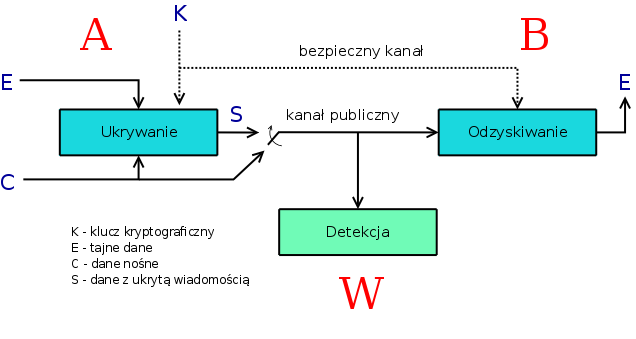
\includegraphics[scale=0.4]{\ImgPath/rys/schemat_komunikacji.png}
% \end{center}
% 	\caption{Schemat komunikacji steganograficznej}
% 	\label{schematKomunikacji}
% \end{figure}

% Przedstawioną tak sytuację pokazuje rysunek 
% \ref{schematKomunikacji}\footnote{sporządzony na podstawie 
% \cite{schematKomunikacjiPrzypis}, rysunek 1, strona 3}. \tech{A} próbuje 
% przesłać tajną informację \tech{E} do \tech{B}. Cała komunikacja odbywa się 
% przez kanał publiczny, kontrolowany przez \tech{W}. W celu ukrycia faktu 
% komunikacji \tech{A} stara się ukryć tajny przekaz w informacji \tech{C}. W celu 
% uzyskania skutecznej steganografii \tech{W} nie może rozróżnić informacji 
% poprawnej, nie zawierającej tajnych danych, od informacji \tech{S}, która 
% zawiera tajną informację. W celu dodatkowego zabezpieczenia przekazu, \tech{A} i 
% \tech{B} mogą korzystać z funkcji kryptograficznej zabezpieczającej przekazywane 
% informacje. Można tu wykorzystać metody kryptografii symetrycznej (ustalony 
% klucz kryptograficzny \tech{K}) lub niesymetrycznej (klucz publiczny 
% \tech{K}$_{pub}$ i klucz prywatny \tech{K}$_{pryw}$).

% Stosowanie technik kryptograficznych wpływa na poprawę bezpieczeństwa 
% przesyłanej informacji, jednak należy pamiętać o nieporządnych cechach jakie 
% mogą one wywołać. W większości przypadków umieszczenie tajnej informacji 
% steganograficznej w przekazie wiąże się z zamianą istniejącej już nieważnej 
% części informacji. Jednak każda porcja usuniętej informacji może mieć pewną 
% charakterystyczną postać lub specyficzny histogram. Zastosowanie funkcji 
% kryptograficznej w stosunku do tajnej informacji zmienia ją, a wynikowy rozkład 
% bitów jest nieprzewidywalny i w większości przypadków różny od standardowych 
% histogramów określonych dla podmienianych części wiadomości.
%   %-----------------
%   % Stegoanaliza
%   %-----------------
% \section{Stegoanaliza}
% Stegoanaliza to nauka zajmująca się wykrywaniem istnienia ukrytych informacji w 
% kanałach komunikacyjnych. Nie zawsze prowadzi to do odkrycia dokładnej treści 
% ukrytego przekazu, a w większości przypadków polega jedynie na wskazaniu 
% istnienia ukrytego kanału steganograficznego.

% Możliwość wykrycia kanału steganograficznego sprowadza się do analizy różnych 
% części wiadomości lub strumienia danych w celu wykrycia anomalii. Takie 
% podejście wynika z faktu, że tajna informacja ukryta jest w miejscach nie 
% przeznaczonych do przesyłania informacji lub na miejscu danych, które są w 
% pewien sposób nadmiarowe (np. dla zmysłów człowieka). Można wskazać dwa 
% podstawowe sposoby wykrywania anomalii:
% \begin{itemize}
% 	\item pierwsze podejście opiera się na przebadaniu wszystkich części 
% informacji (np. pól nagłówka TCP/IP), których struktura jest w pełni 
% przewidywalna lub których wartości są zdefiniowane przez standardy lub 
% powszechne praktyki; ważne jest także sprawdzenie czy występują wartości 
% nadmiarowe oraz czy elementy sygnalizujące wystąpienie dodatkowych danych mają 
% faktyczne pokrycie w danych,
% 	\item drugą metodą jest porównanie wartości części wiadomości (np. pól 
% nagłówka TCP/IP) i zaklasyfikowanie ich jako prawdopodobnych lub nie dla danego 
% systemu bądź protokołu; takie podejście może być stosowane do wartości ściśle 
% określonych, takich jak wymienione w pierwszym punkcie, jednak można je także 
% stosować do wartości które są pseudolosowe lub których histogram jest 
% charakterystyczny; w celu realizacji tej metody warto posłużyć się sieciami 
% neuronowymi takimi jak SVM i RSVM, zdolnymi rozpoznawać wzorce i separować dane.
% \end{itemize}
%   %-----------------
%   % Metody tworzenia steganografii
%   %-----------------
% \section{Metody tworzenia steganografii oraz rodzaje ukrytych kanałów}
% Przesłanie danych za pomocą przekazu steganograficznego wiąże się w większości 
% przypadków z umieszczeniem dodatkowej informacji w wiadomości. Odbywa się to za 
% pomocą podmiany tej części wiadomości (nagłówka TCP/IP), która wykazuje cechy 
% nadmiarowości lub której (kontrolowana) zmiana nie prowadzi do przerwania 
% transmisji. Pewną podgrupą może być w tym przypadku wykorzystanie pól 
% oryginalnie pustych (zerowych) lub niewykorzystywanych w istniejących 
% implementacjach.

% Kanały steganograficzne można podzielić na dwa zasadniczne 
% typy\cite{SweetyPresentation}:
% \begin{itemize}
% 	\item kanał pojemnościowy (ang. storage channel) - informacja zawarta w 
% częściach wiadomości, polach nagłówka,
% 	\item kanał czasowy (ang. timing channel) - informacja zawarta w czasach 
% wystąpienia danych zdarzeń, np. przesłania pakietu TCP/IP.
% \end{itemize}
% W przypadku sieci pakietowych można także połączyć dwa typu kanałów 
% steganograficznych, tworząc kanał mieszany, w którym jeden z typów (np. 
% pojemnościowy) będzie wykorzystywany do przekazywania informacji, a drugi (np. 
% czasowy) do sygnalizacji tego zdarzenia.

% Większość opracowanych programów służących do przesyłania danych z 
% wykorzystaniem steganografii opiera się na kanałach pojemnościowych. Wynika to z 
% faktu, że kanały czasowe narzucają pewne ograniczenia na generację pakietów 
% TCP/IP przez co ich wykrycie staje się prostsze.

% Dodatkowo należy zauważyć, że w sieciach pakietowych można skonstruować 
% abstrakcyjny kanał steganograficzny, w którym do przesyłania tajnych danych 
% lub/i obsługi protokołu steganograficznego wykorzystywane są różne pola 
% nagłówka. Zmiana wykorzystania danego pola może być dynamiczna, zależna od 
% wymaganej przepustowości lub w celu zminimalizowania wykrycia kanału 
% steganograficznego. 
%   %-----------------
%   % Cechy kanału steganograficznego
%   %-----------------
% \section{Cechy kanału steganograficznego}
% Każdy kanał steganograficzny posiada trzy cechy, które decydują o jego 
% przydatności w danej sytuacji:
% \begin{enumerate}
% 	\item pojemność (przepustowość) - określa jaką porcję informacji możemy 
% przesłać w danej wiadomości nośnej; w przypadku steganografii w TCP/IP, wyrażana 
% jest w bitach na sekundę, bitach na pakiet lub bitach na sesję TCP; 
% przepustowość odgrywa ważną rolę w przypadku konieczności przekazania dużej 
% ilości informacji, jednak należy pamiętać, że to przeważnie prowadzi do 
% ułatwionej detekcji steganografii,
% 	\item bezpieczeństwo - określa jak łatwo jest uzyskać dostęp do 
% przekazywanej tajnej informacji w przypadku poznania mechanizmu tworzenia 
% przekazu steganograficznego; dodatkowym mechanizmem zwiększającym bezpieczeństwo 
% może być używanie znanych tylko sobie zmiennych pseudolosowych lub modyfikacji 
% algorytmu\footnote{jest to znane jako ,,bezpieczeństwo przez zatajenie'' (ang. 
% security through obscurity) i powinno być używane tylko jako dodatkowy element 
% systemu zabezpieczeń},
% 	\item krzepkość (ang. robustness) - określa stopień w jakim możemy 
% zmodyfikować przekaz nie uszkadzając zawartej w nim informacji 
% steganograficznej; niestety w przypadku steganografii naruszenie kanału (pola) 
% zawierającego przekaz steganograficzny przeważnie wiąże się z utratą tajnego 
% przekazu.
% \end{enumerate}

%   %-----------------
%   % Steganografia w obiektach multimedialnych
%   %-----------------
% \section{Steganografia w obiektach multimedialnych}
% \label{sectionSteganografiaWObiektachMultimedialnych}
% Pomimo, że steganografia ma zastosowanie prawie w każdej formie komunikacji, w 
% latach 90-tych zyskała ona powodzenie jako technika ukrywania informacji w 
% obiektach multimedialnych. Wynika to przede wszystkim z powszechności tego 
% rodzaju przekazu, jego rozmiarów oraz prostoty obsługi programów do ukrywania 
% informacji w obiektach multimedialnych, takich jak obraz, dźwięk i wideo. 
% Dodatkowym atutem przy zastosowaniu tych metod jest stosunek ukrytej informacji 
% do oryginalnego przekazu, sięgający w ekstremalnych sytuacjach 50\%, bez 
% zauważalnego pogorszenia się jakości przekazywanych danych.

% Użycie steganografii w treściach multimedialnych sprowadza się do takiego 
% manipulowania danymi, aby plik wynikowy zawierał dodatkowe informacje, a 
% jednocześnie nie był rozróżniany przez zmysły człowieka w porównaniu z 
% oryginałem.

% Jedną z najszerzej omawianych form steganografii w obiektach multimedialnych 
% jest ukrywanie informacji w plikach graficznych. Istnieje wiele rozwiązań, 
% zarówno bezpłatnych, o otwartym kodzie jak i komercyjnych. Przykładami mogą tu 
% być takie programy jak Outguess, JPHide, StegHide. Istnieją różne techniki 
% ukrywania informacji w plikach graficznych. Najprostszym rozwiązaniem jest 
% podmiana najmniej znaczących bitów opisujących kolor danego piksela. Możliwe 
% jest też zastosowanie dyskretnej transformaty kosinusowej.

% W przypadku wybrania jako wiadomości nośnej pliku audio, możemy także zastosować 
% metodę podmiany najmniej znaczących bitów. Dodatkowo stosowane są metody 
% ukrywania tajnych wiadomości poprzez rozszerzanie spektrum danego nagrania, czy 
% też dodawanie echa. Przykładem narzędzia do tworzenia wiadomości 
% steganograficznych może być UnderMP3Cover, MP3Stego czy 
% S-Tools\footnote{\url{http://www.stegoarchive.com}}.

% Kolejnym przykładem wykorzystania jako pliku nośnego obiektu multimedialnego 
% jest plik wideo. Dodatkowa informacja może być przekazana przy użyciu dyskretnej 
% transformaty kosinusowej. Jako przykładowe implementacje można podać StegoVideo.

% Istnieje kilka technik umożliwiających wykrycie lub usunięcie steganografii 
% zastosowanej w obiektach multimedialnych. Pierwszym podejściem, choć przeważnie 
% trudnym do zastosowania, jest użycie oryginalnego pliku jako wzorca do 
% porównania z przechwyconą wersją. W przypadku plików graficznych lub wideo 
% możliwe jest użycie analizatorów statystycznych, które mogą wykryć anomalie 
% występujące w histogramach tych wiadomości.

% Zamiast wykrywać istnienie steganografii, częstym podejściem jest jej 
% ograniczanie lub ,,ślepe'' usuwanie z wiadomości tych danych, które mogą być 
% nośnikiem kanału steganograficznego. W przypadku plików multimedialnych 
% najlepszym sposobem uzyskania takiego efektu jest przekodowanie pliku na inny 
% standard i powrót do standardu wejściowego. Przeważnie zmiany w jakości plików 
% są niezauważalne, a użycie konwersji sprowadza się do takiej zmiany bitów, która 
% niszczy zawartą w nich steganografię.

% W przypadku plików multimedialnych użycie steganografii jest pomocne w ochronie 
% praw autorskich, przez stosowanie jej jako cyfrowych znaków wodnych. Niestety, 
% tak jak zostało to wcześniej przedstawione w trakcie konwersji wiele z 
% zakodowanej informacji ginie bezpowrotnie. Skutkiem tego może być pogorszenie 
% jakości pliku multimedialnego, ale także usunięcie z niego cyfrowego znaku 
% wodnego.

% Itd., itd., itd. ...

% \chapter{Steganografia w ruchu TCPIP}
% \label{chapterSteganografiaWRuchuTCPIP}

% Itd., itd., itd ...

%-----------------
% Wnioski 
%-----------------
\chapter{Wnioski}

% Protokół TCP/IP jest najbardziej rozpowszechnionym i używanym protokołem 
% komunikacji między systemami w sieci Internet oraz w sieciach intranet. Niestety 
% został on opracowany na początku lat siedemdziesiątych, gdy problemy 
% bezpieczeństwa informacji nie stały na pierwszym miejscu. Ciągły wzrost działań 
% przestępczych w sieci Internet, w tym wymiana nielegalnych treści, prowadzi do 
% stosowania coraz to nowszych technik zabezpieczających. Z tego względu obserwuje 
% się działania mające na celu wprowadzenie tajnej komunikacji między przejętymi 
% systemami, tak aby nie wzbudzić ostrzeżeń w analizatorach sieciowych. Taka 
% ukryta komunikacja odbywa się z wykorzystaniem steganografii.

% Wprowadzenie steganografii do niskich warstwach stosu TCP/IP umożliwia obejście 
% wielu filtrów nałożonych na warstwy wyższe. Większość sieci oparta jest na 
% protokołach rodziny TCP/IP, przez co nie można zabronić ich używania. Możliwa 
% jest jedynie kontrola poprawności semantyki protokołów TCP/IP, a także 
% ewentualna ingerencja w przekazywane wartości, z uwzględnieniem stanowości 
% niektórych pól.

% Opracowany schemat generacji początkowych numerów sekwencyjnych w jak najlepszy 
% sposób odzwierciedla oryginalny proces zachodzący w stosie sieciowym systemu 
% Linux. W większości przypadków występujących w rzeczywistych sieciach i 
% systemach, numery wygenerowane przy pomocy \tech{Shushi} nie byłyby rozróżnialne 
% od numerów wygenerowanych przez stos sieciowy systemu.

% Jeżeli proces generacji wartości użytych do przekazania danych 
% steganograficznych zostanie oparty o oryginalne mechanizmy używane do ich 
% generacji, to pasywny analizator sieciowy nie będzie w stanie wykryć istnienia 
% anomalii. Różnice możliwe są do zaobserwowania w przypadku zaistnienia 
% specyficznych sytuacji występujących dla danej implementacji protokołu. W 
% przypadku zastosowania pasywnego analizatora wymaga to jednak oczekiwania na 
% taką sytuację. Z przeprowadzonych testów wynika, że lepszym podejściem jest 
% zastosowanie analizatorów aktywnych, które posiadają wiedzę na temat testowanych 
% systemów oraz ich chrakterystycznych cech implementacji. Skonstruowanie takiego 
% analizatora jest zadaniem stosunkowo prostym a daje bardzo wysoką skuteczność.

% Z przeprowadzonych testów wynika, że celowe jest prowadzenie dalszych prac w 
% następujących obszarach:
% \begin{itemize}
%  \item dokładniejszy mechanizm generacji wartości mikrosekund
%  \item wprowadzenie algorytmów zdolnych wykryć i uniemożliwić działanie 
% analizatora aktywnego
% \end {itemize}

% Jeżeli powyższe punkty nie zostaną spełnione, analizatory aktywne będą w stanie 
% wykryć istnienie modułu steganograficznego opartego na początkowych numerach 
% sekwencyjnych.

% \begin{tabular}{c|cc}
% pierwsza kolumna & druga & trzecia \\ \hline
% 1 & 2 & 3 \\
% a & b & c \\
% \end{tabular} 

% \begin{equation}
%  E = m c^2 \label{einstein}
% \end{equation}

% Rozwój opracowanego rozwiązania steganograficznego jest możliwy poprzez 
% wprowadzenie elementów  -- patrz wzór (\ref{einstein}) -- jak:
% \begin{itemize}
%  \item obsługa innych, przyszłościowych protokołów sieciowych, takich jak SCTP 
% (ang. Stream Control Transmission Protocol)\cite{RFC2960}
%  \item zapewnienie dwustronnej komunikacji z wykorzystaniem numerów 
% potwierdzenia \tech{ACK}
%  \item przeniesienie implementacji do innych systemów operacyjnych
% \end{itemize}

% Wraz ze wzrostem przepustowości urządzeń sieciowych (obecnie 10Gb/s i więcej) 
% wzrasta problem analizy przepływających danych w czasie rzeczywistym. 
% Analizatory sieciowe muszą w coraz krótszym czasie zbadać coraz większy strumień 
% danych (miliony pakietów na sekundę). Jednak problem wzrostu prędkości sieci 
% utrudnia zadanie także osobom implementującym kanały steganograficzne w 
% protokole TCP/IP. Coraz więcej operacji wyższych warstw stosu sieciowego 
% przenoszonych jest do układów scalonych interfejsów sieciowych. Taka technologia 
% znana jest pod skrótem TOE (ang. TCP Offload Engine) i odnosi się przede 
% wszystkim do sprzętowej generacji sum kontrolnych oraz mechanizmu TSO (ang. TCP 
% segmentation offload). W następnych latach spodziewane jest przenoszenie 
% kolejnych elementów stosu sieciowego TCP/IP do implementacji sprzętowych.

% Ze względu na rozwój systemów zabezpieczających ruch sieciowy oraz wzrost 
% bezpieczeństwa systemów operacyjnych, w kolejnych latach wzrośnie także 
% wykorzystanie technik steganograficznych przez grupy przestępcze działające w 
% ramach Internetu. Z tego powodu poznanie technik steganograficznych oraz 
% wypracowanie metod obrony i wykrywania takiej komunikacji jest bardzo ważne.

%-----------------
% Dodatki 
%-----------------
% \appendix
% \chapter{Porównanie numerów ISN jądra Linux i modułu Shushi}
% \begin{figure}[!htbp]
% 	\begin{center}
% \centering
% 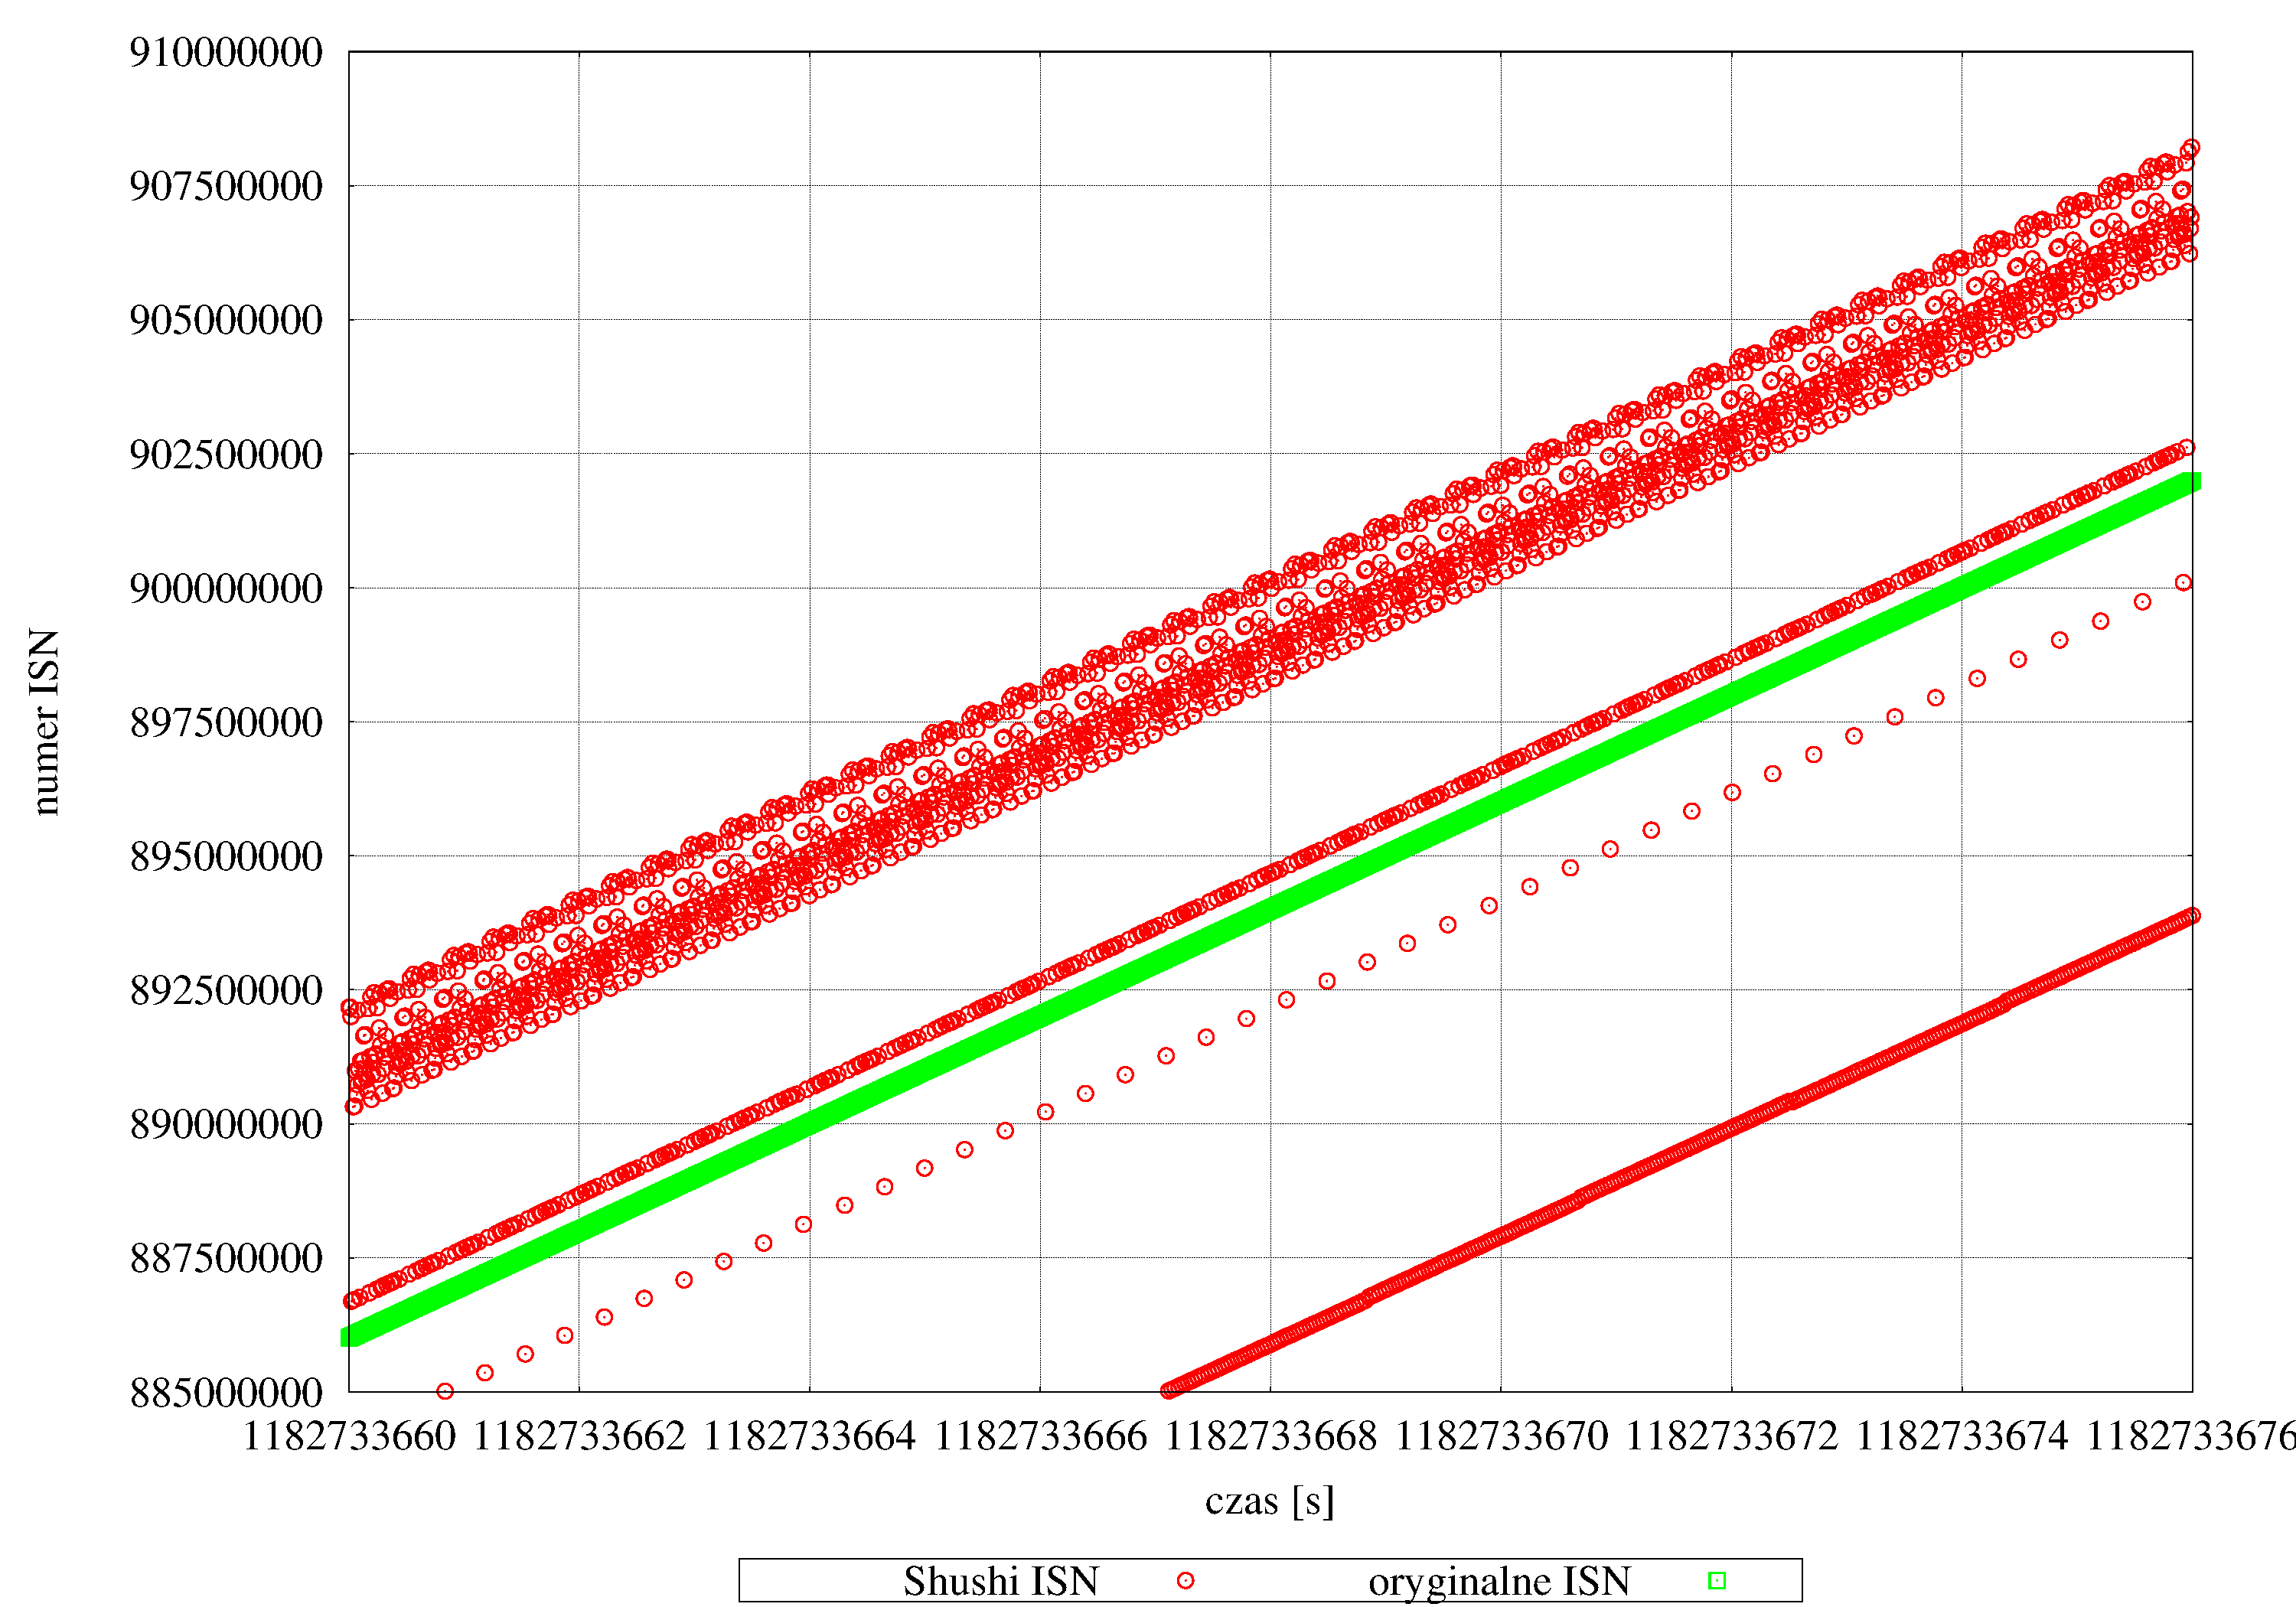
\includegraphics[scale=0.21]{\ImgPath/rys/IPPortConstData.pdf}
% \end{center}
% 	\caption{Numery ISN wygenerowane przez jądro oraz \tech{Shushi}, stałe 
% numery IP oraz porty TCP, stałe dane dla \tech{Shushi}, serie po około 2800 
% próbek.}
% 	\label{IPPortConstData}
% \end{figure}

% \begin{figure}[!htbp]
% 	\begin{center}
% \centering
% 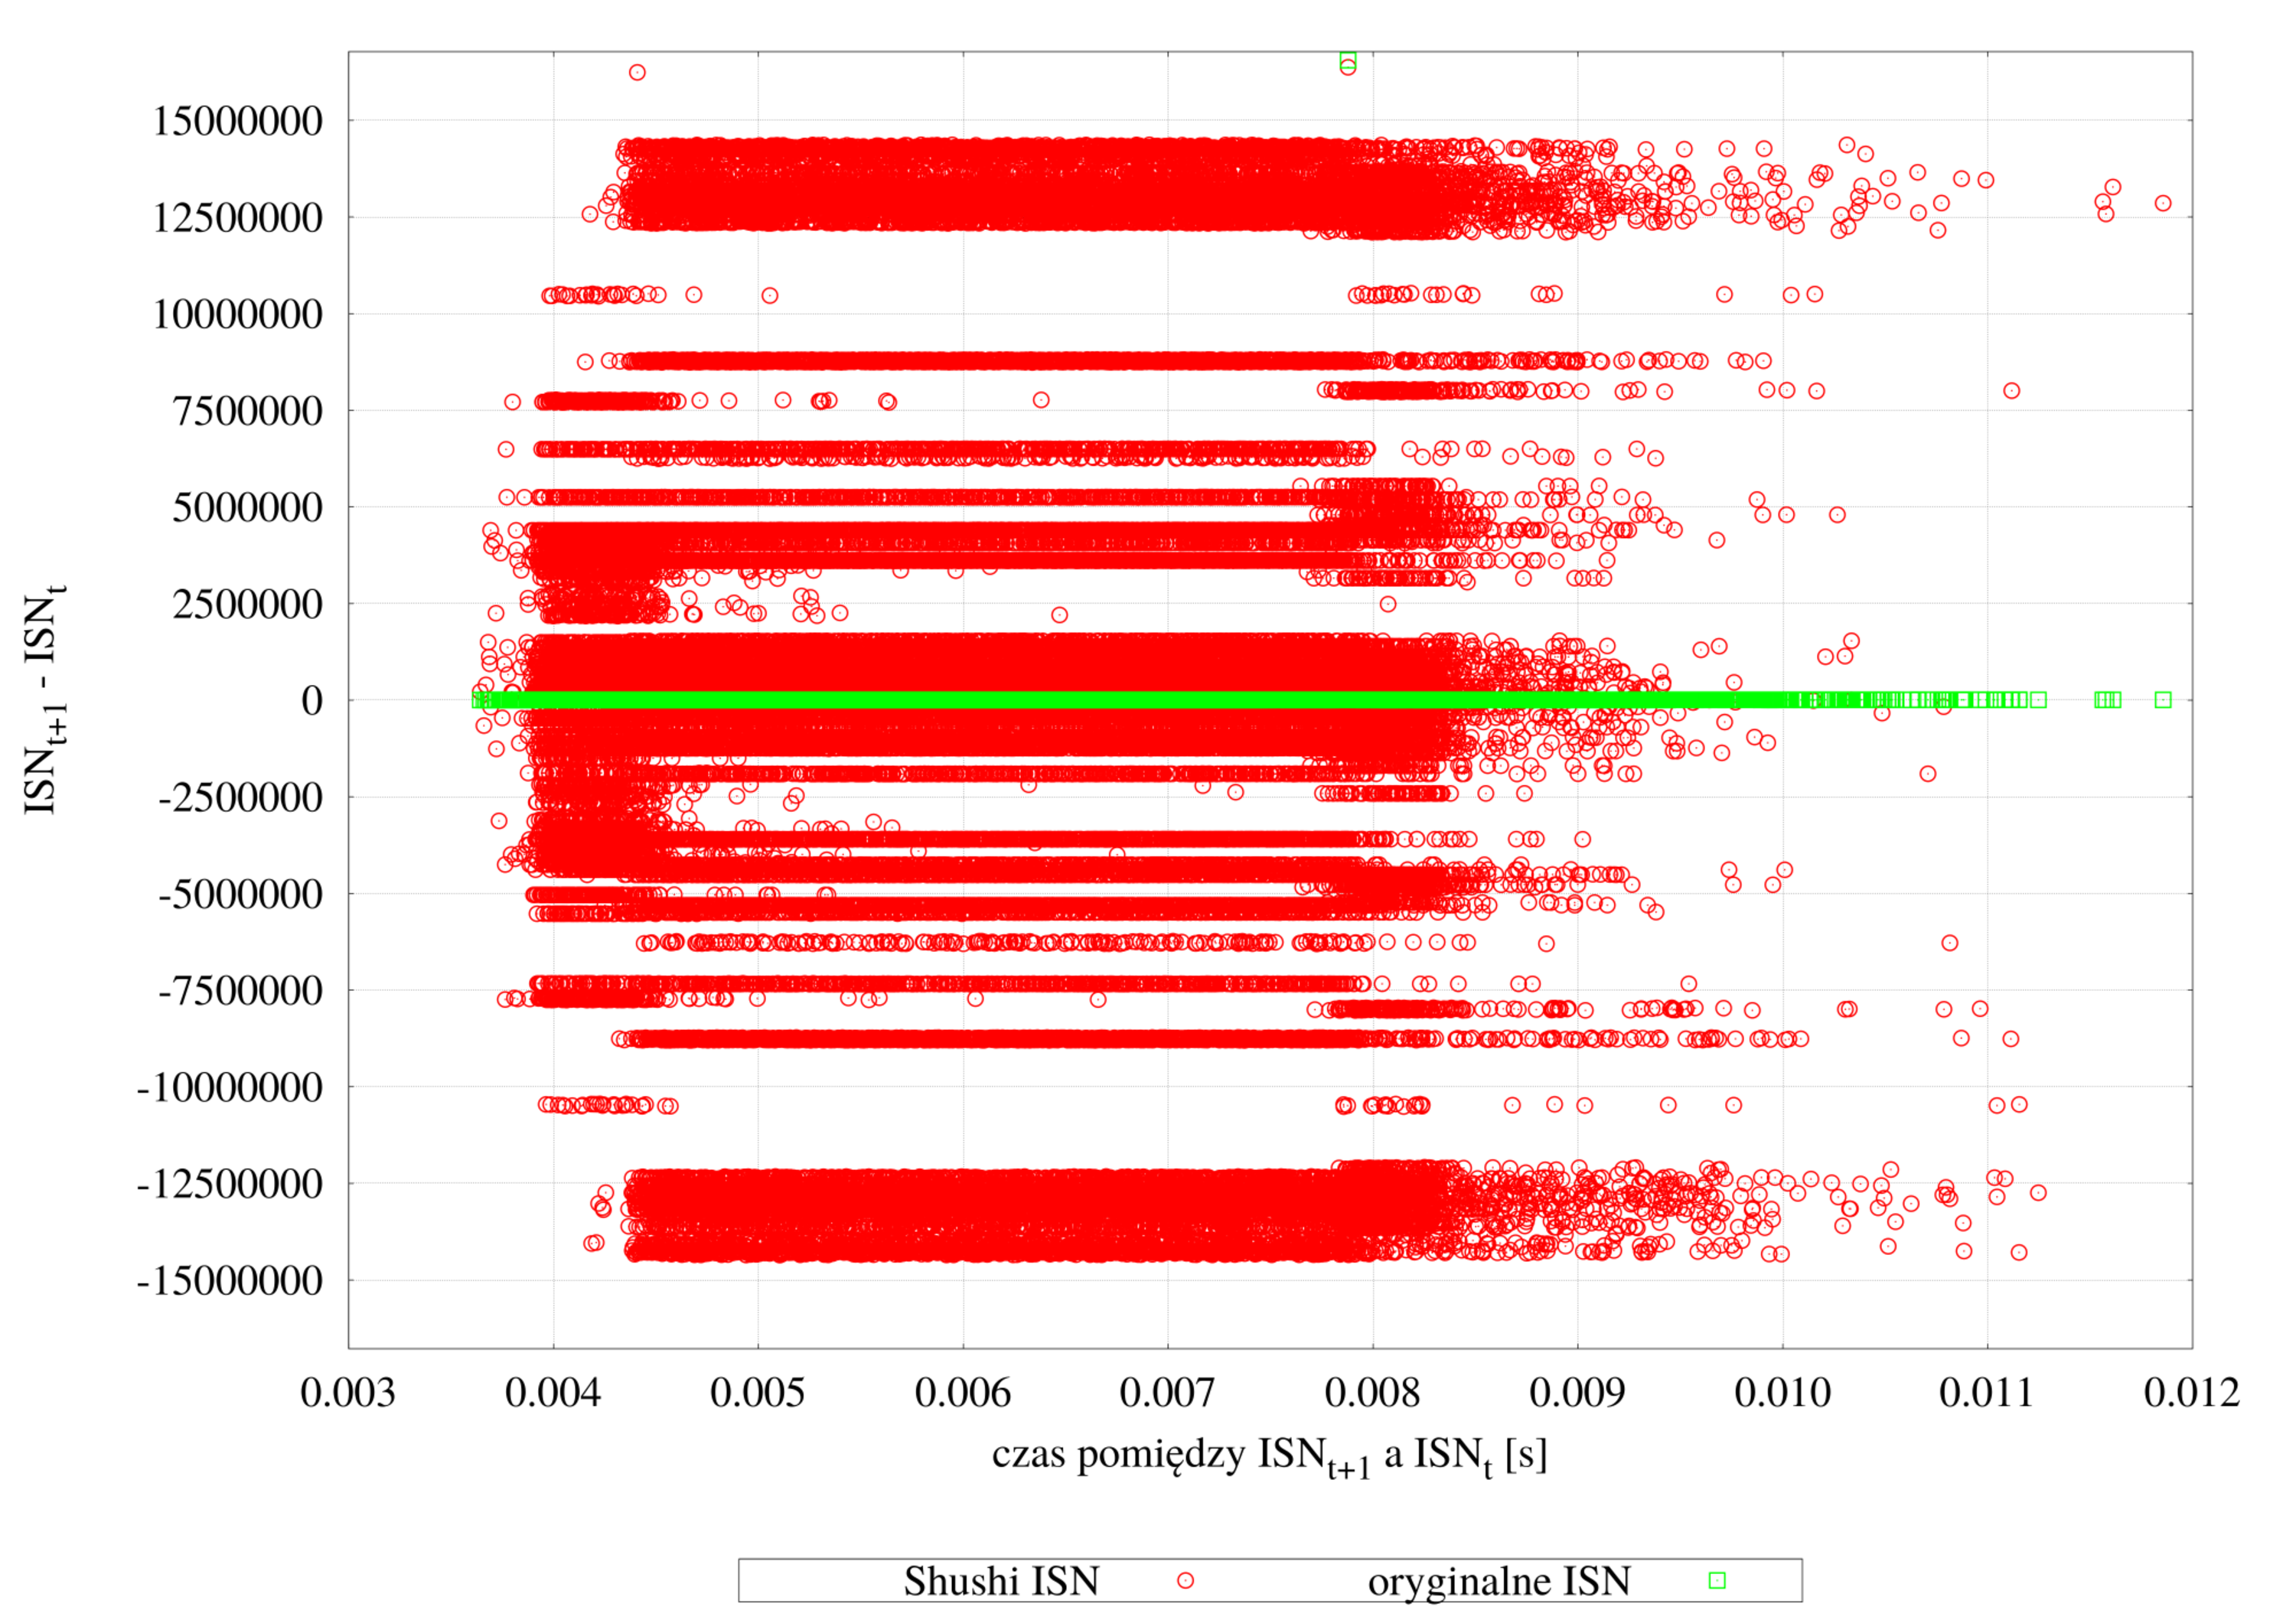
\includegraphics[scale=0.21]{\ImgPath/rys/IPPortConstDataDiff.pdf}
% \end{center}
% 	\caption{Różnice pomiędzy kolejnymi numerami ISN wygenerowanymi przez 
% jądro oraz \tech{Shushi}, stałe numery IP oraz porty TCP, stałe dane dla 
% \tech{Shushi}, serie po około 60000 próbek.}
% 	\label{IPPortConstDataDiff}
% \end{figure}

% \begin{figure}[!htbp]
% 	\begin{center}
% \centering
% 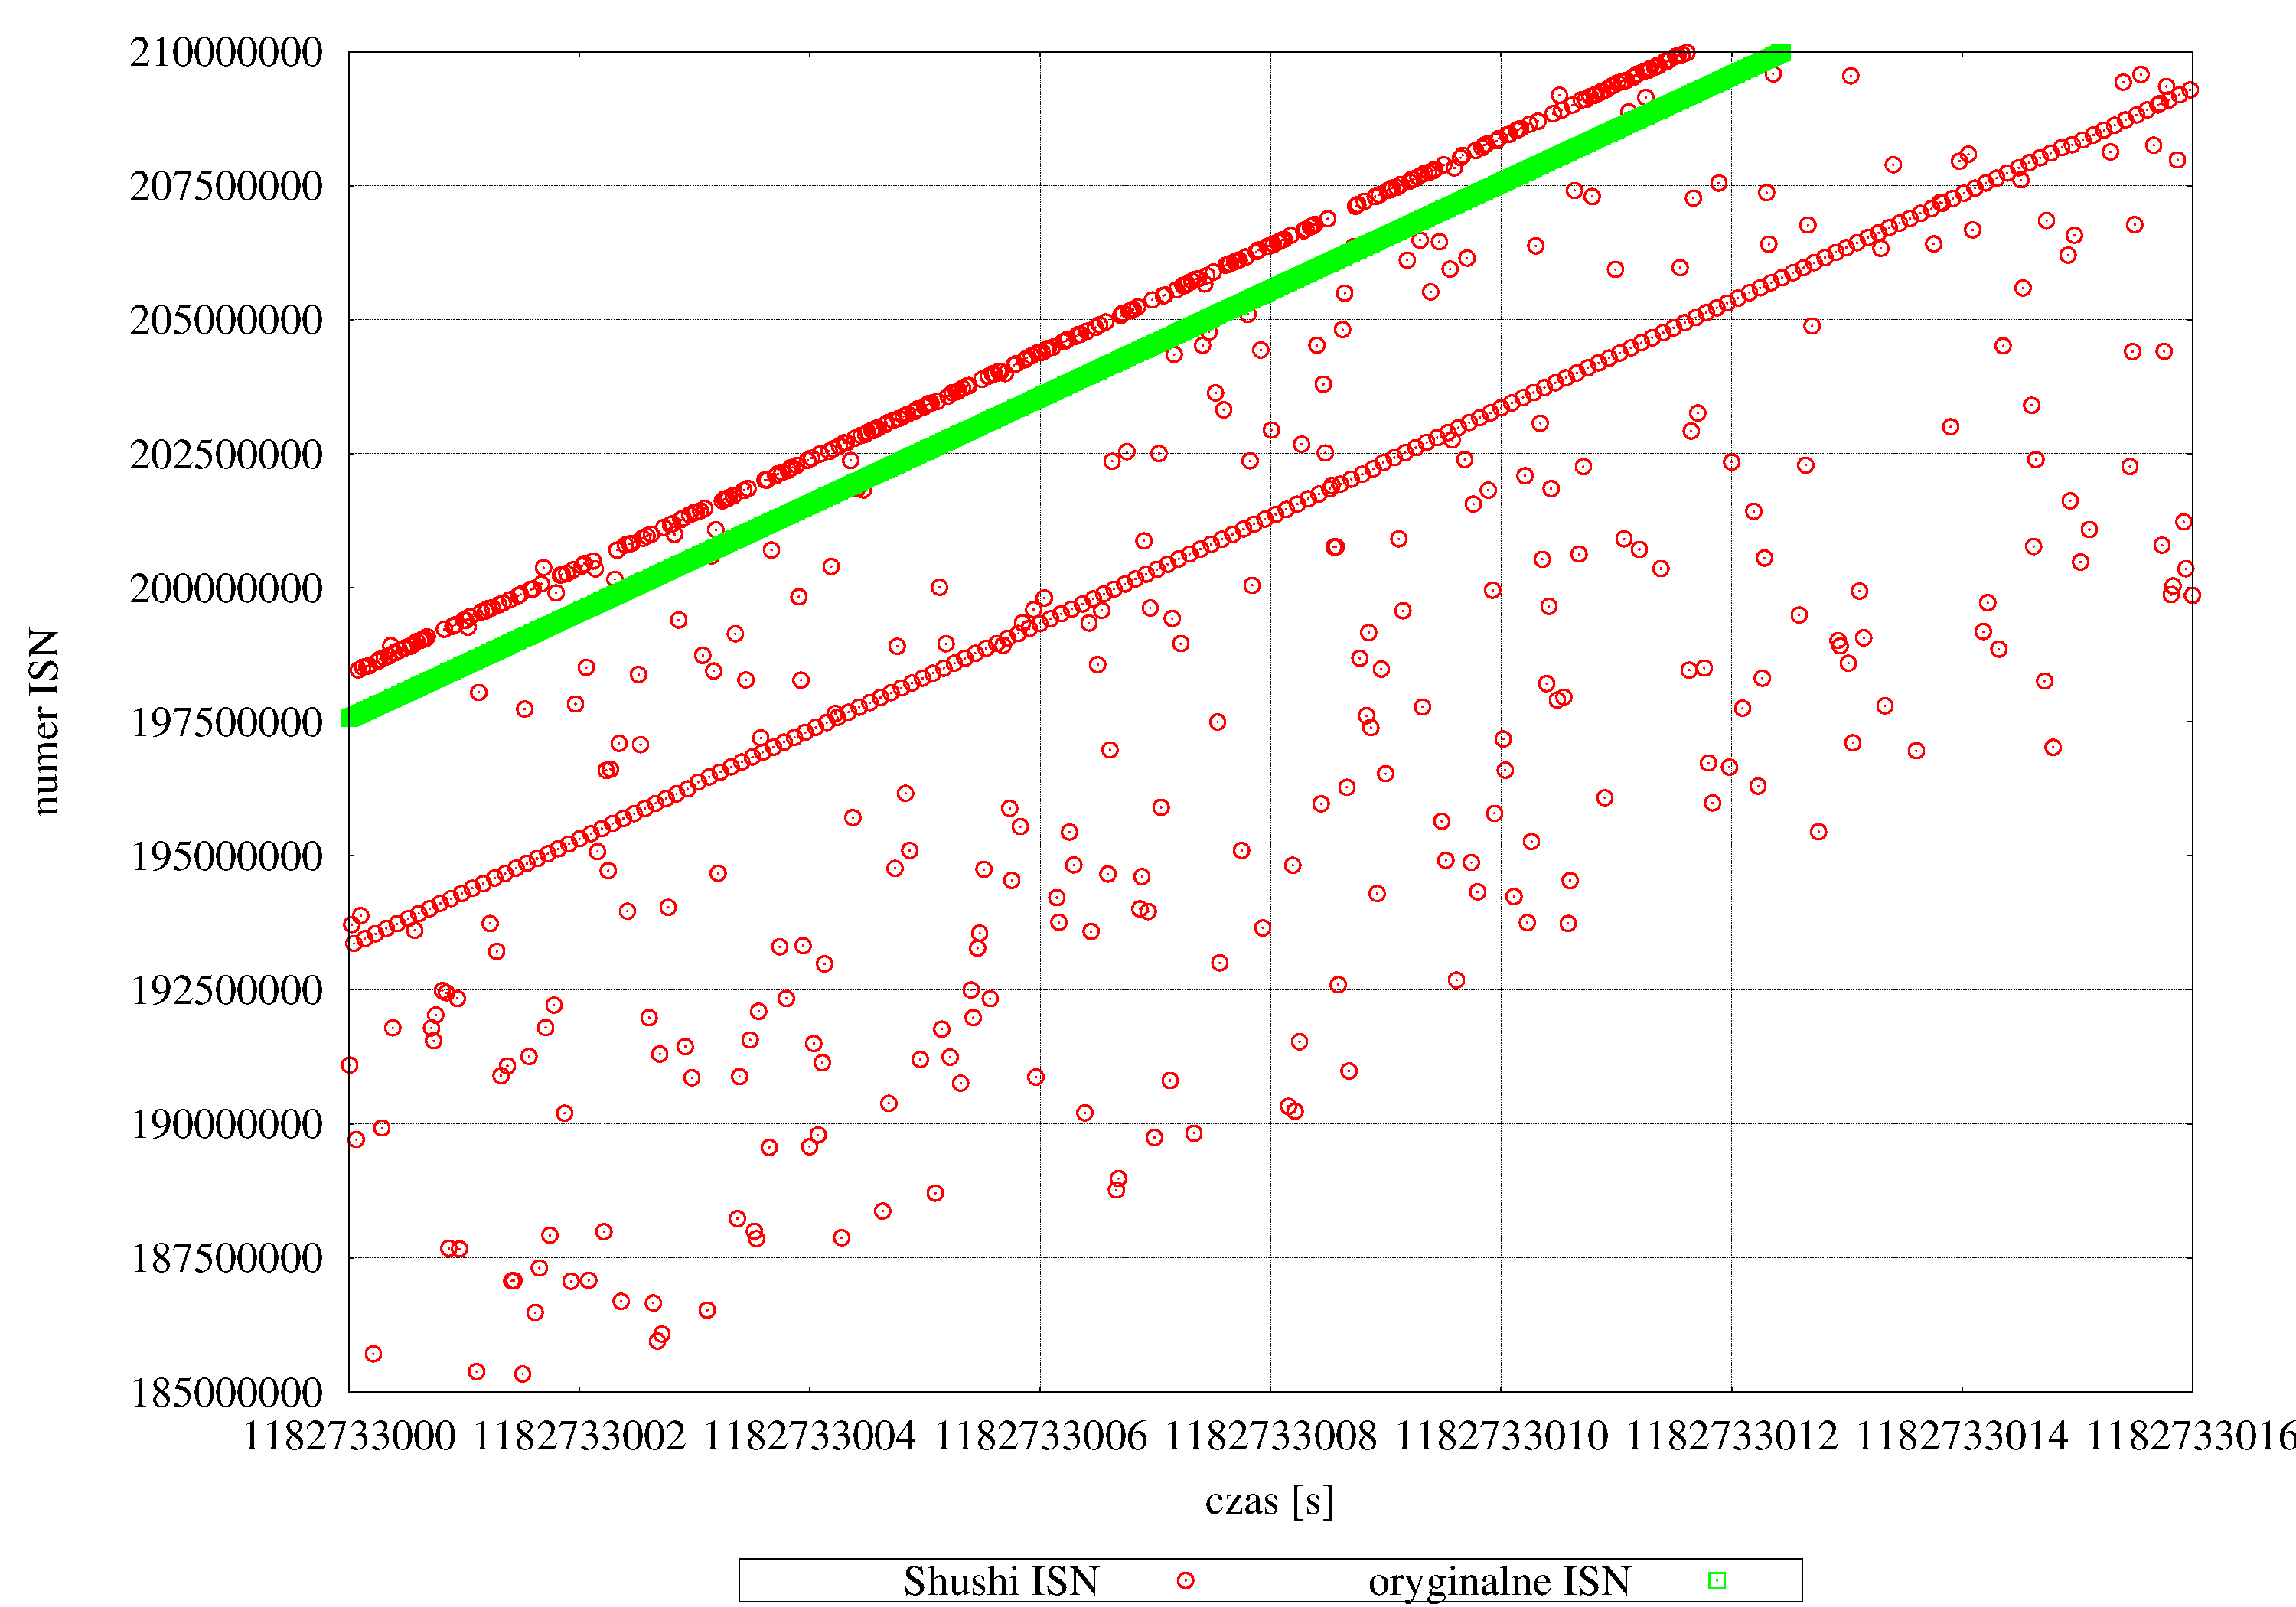
\includegraphics[scale=0.21]{\ImgPath/rys/IPPortRandData.pdf}
% \end{center}
% 	\caption{Numery ISN wygenerowane przez jądro oraz \tech{Shushi}, stałe 
% numery IP oraz porty TCP, losowe dane dla \tech{Shushi}, serie po około 860 
% próbek.}
% 	\label{IPPortRandData}
% \end{figure}

% \begin{figure}[!htbp]
% 	\begin{center}
% \centering
% 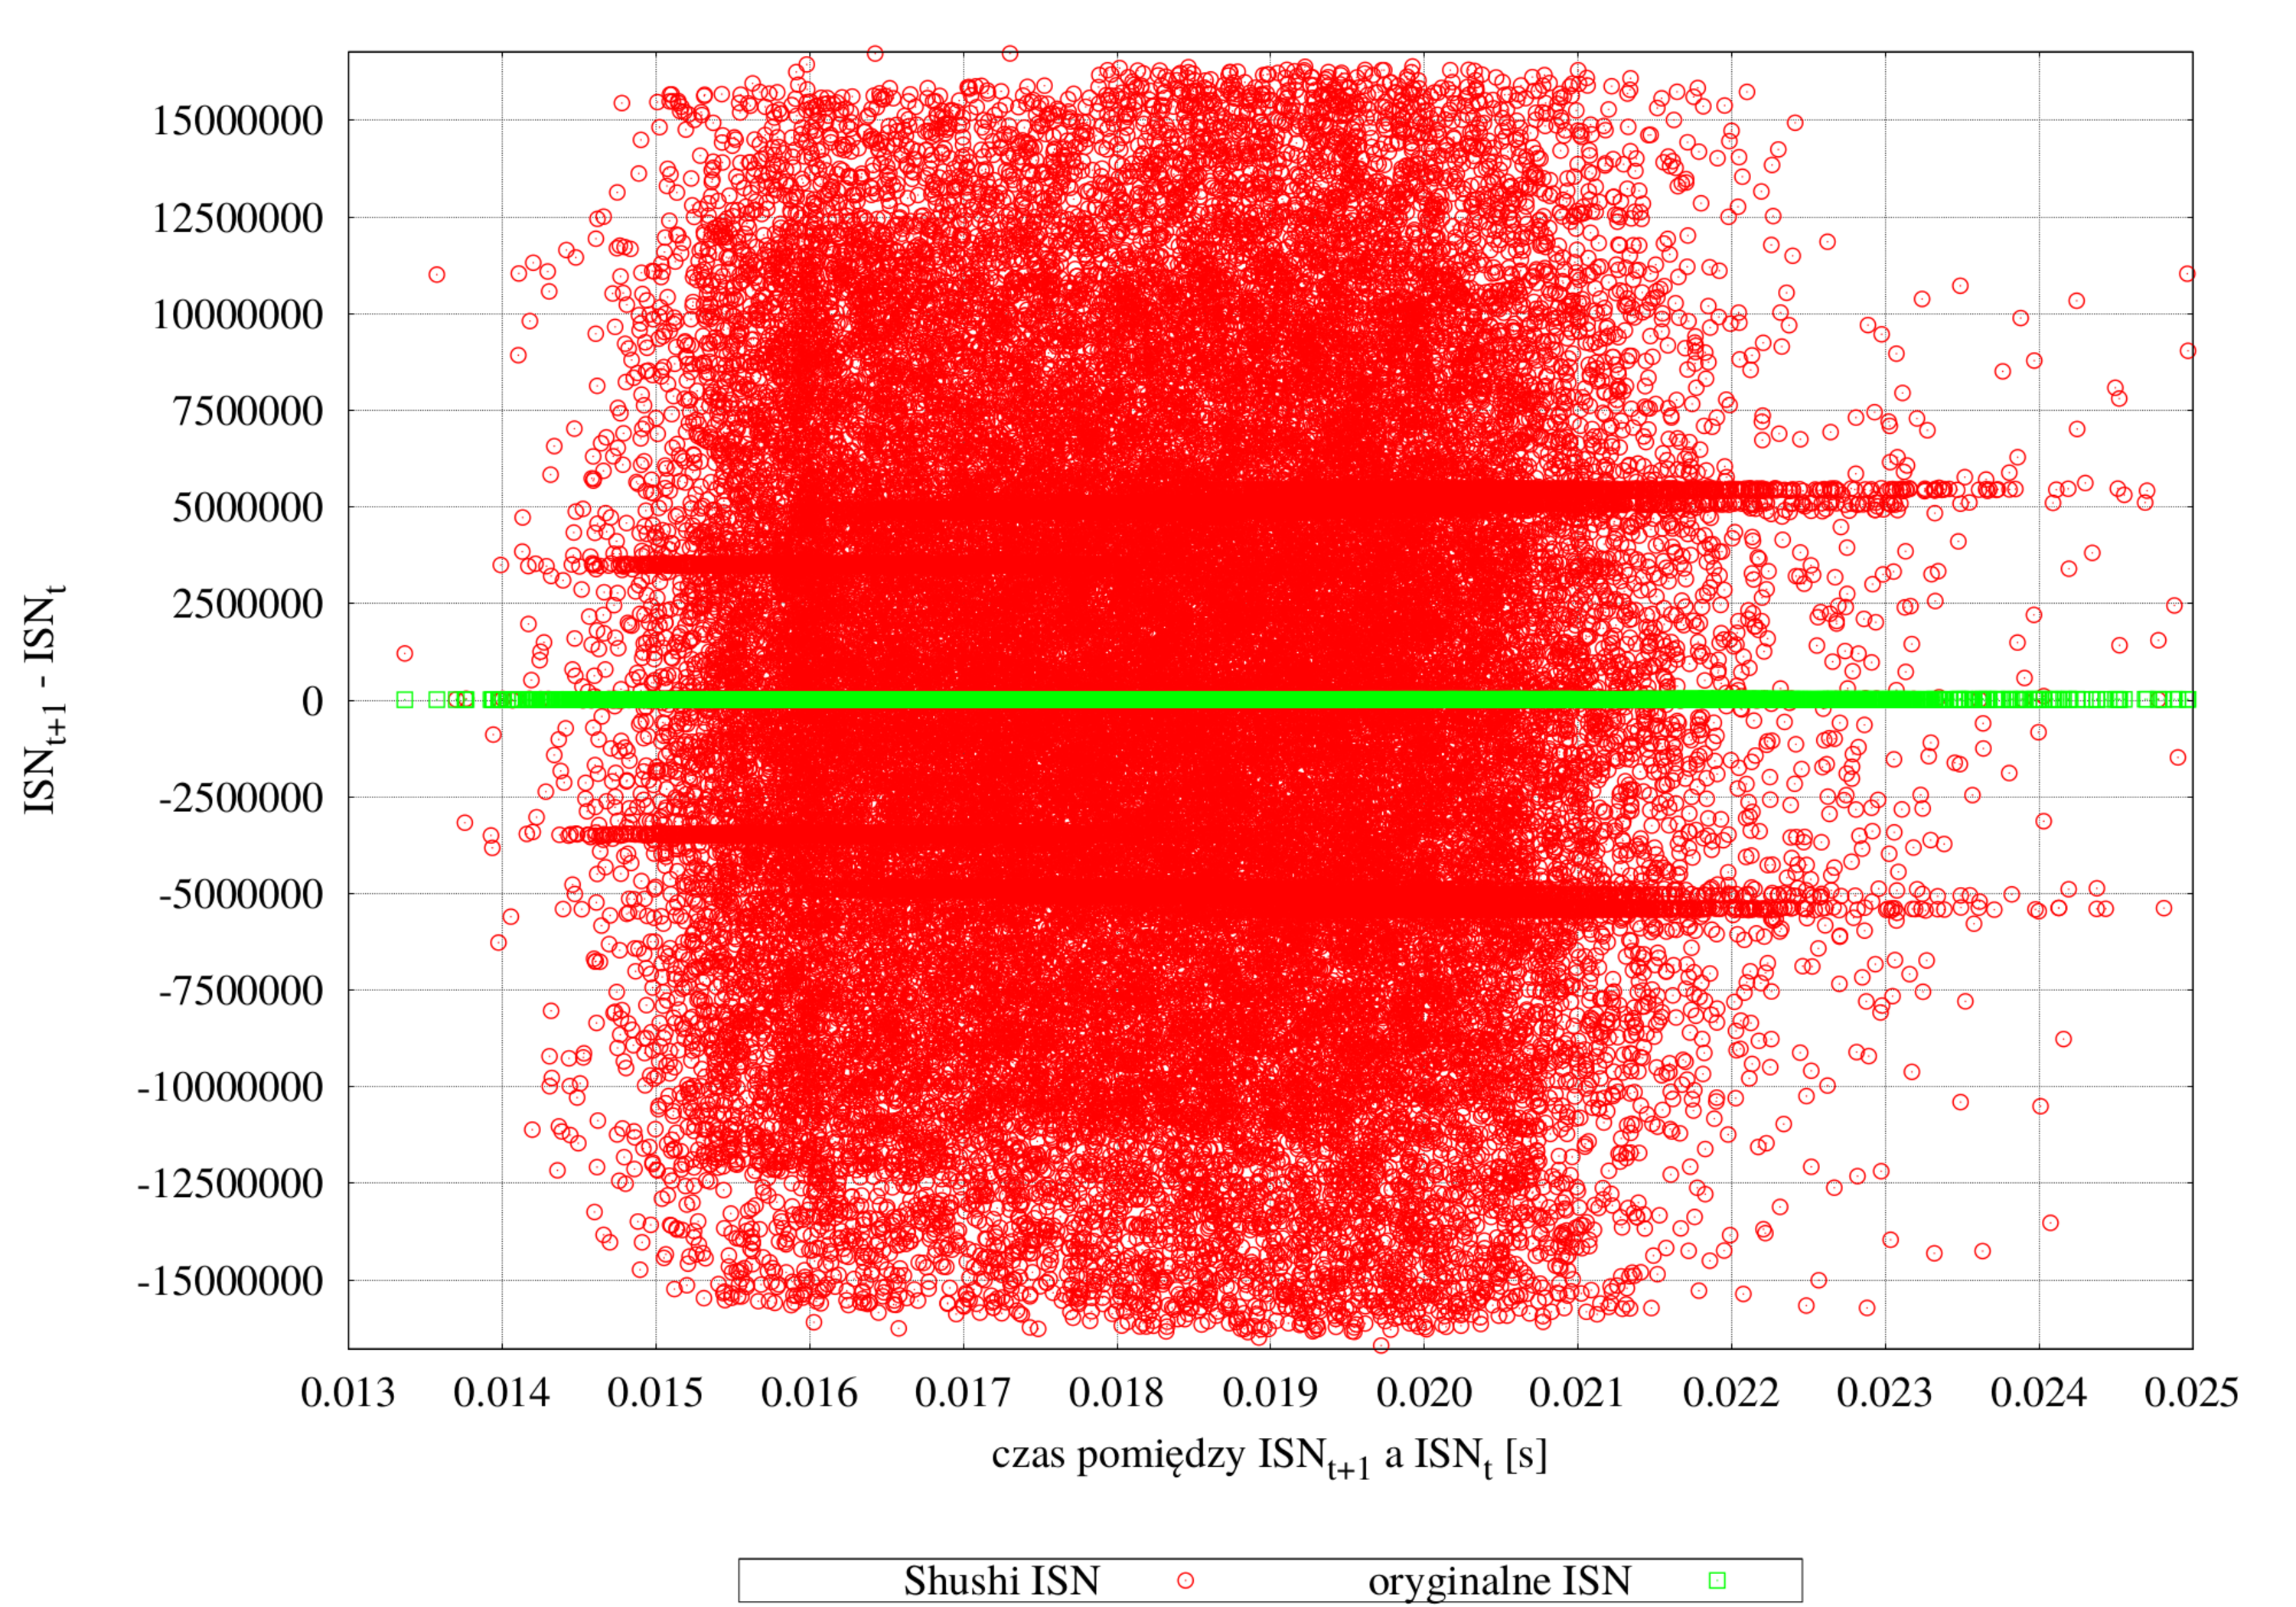
\includegraphics[scale=0.21]{\ImgPath/rys/IPPortRandDataDiff.pdf}
% \end{center}
% 	\caption{Różnice pomiędzy kolejnymi numerami ISN wygenerowanymi przez 
% jądro oraz \tech{Shushi}, stałe numery IP oraz porty TCP, losowe dane dla 
% \tech{Shushi}, serie po około 60000 próbek.}
% 	\label{IPPortRandDataDiff}
% \end{figure}

% \begin{thebibliography}{99}

\bibliographystyle{acm}
\bibliography{./bibliografia}
\addcontentsline{toc}{chapter}{Bibliografia}


\zakonczenie  % wklejenie recenzji i opinii

\end{document}
%+++ END +++
